% Options for packages loaded elsewhere
\PassOptionsToPackage{unicode}{hyperref}
\PassOptionsToPackage{hyphens}{url}
\PassOptionsToPackage{dvipsnames,svgnames,x11names}{xcolor}
%
\documentclass[
  letterpaper,
  number,
  review,
  3p]{elsarticle}

\usepackage{amsmath,amssymb}
\usepackage{iftex}
\ifPDFTeX
  \usepackage[T1]{fontenc}
  \usepackage[utf8]{inputenc}
  \usepackage{textcomp} % provide euro and other symbols
\else % if luatex or xetex
  \usepackage{unicode-math}
  \defaultfontfeatures{Scale=MatchLowercase}
  \defaultfontfeatures[\rmfamily]{Ligatures=TeX,Scale=1}
\fi
\usepackage{lmodern}
\ifPDFTeX\else  
    % xetex/luatex font selection
\fi
% Use upquote if available, for straight quotes in verbatim environments
\IfFileExists{upquote.sty}{\usepackage{upquote}}{}
\IfFileExists{microtype.sty}{% use microtype if available
  \usepackage[]{microtype}
  \UseMicrotypeSet[protrusion]{basicmath} % disable protrusion for tt fonts
}{}
\makeatletter
\@ifundefined{KOMAClassName}{% if non-KOMA class
  \IfFileExists{parskip.sty}{%
    \usepackage{parskip}
  }{% else
    \setlength{\parindent}{0pt}
    \setlength{\parskip}{6pt plus 2pt minus 1pt}}
}{% if KOMA class
  \KOMAoptions{parskip=half}}
\makeatother
\usepackage{xcolor}
\setlength{\emergencystretch}{3em} % prevent overfull lines
\setcounter{secnumdepth}{5}
% Make \paragraph and \subparagraph free-standing
\makeatletter
\ifx\paragraph\undefined\else
  \let\oldparagraph\paragraph
  \renewcommand{\paragraph}{
    \@ifstar
      \xxxParagraphStar
      \xxxParagraphNoStar
  }
  \newcommand{\xxxParagraphStar}[1]{\oldparagraph*{#1}\mbox{}}
  \newcommand{\xxxParagraphNoStar}[1]{\oldparagraph{#1}\mbox{}}
\fi
\ifx\subparagraph\undefined\else
  \let\oldsubparagraph\subparagraph
  \renewcommand{\subparagraph}{
    \@ifstar
      \xxxSubParagraphStar
      \xxxSubParagraphNoStar
  }
  \newcommand{\xxxSubParagraphStar}[1]{\oldsubparagraph*{#1}\mbox{}}
  \newcommand{\xxxSubParagraphNoStar}[1]{\oldsubparagraph{#1}\mbox{}}
\fi
\makeatother


\providecommand{\tightlist}{%
  \setlength{\itemsep}{0pt}\setlength{\parskip}{0pt}}\usepackage{longtable,booktabs,array}
\usepackage{calc} % for calculating minipage widths
% Correct order of tables after \paragraph or \subparagraph
\usepackage{etoolbox}
\makeatletter
\patchcmd\longtable{\par}{\if@noskipsec\mbox{}\fi\par}{}{}
\makeatother
% Allow footnotes in longtable head/foot
\IfFileExists{footnotehyper.sty}{\usepackage{footnotehyper}}{\usepackage{footnote}}
\makesavenoteenv{longtable}
\usepackage{graphicx}
\makeatletter
\def\maxwidth{\ifdim\Gin@nat@width>\linewidth\linewidth\else\Gin@nat@width\fi}
\def\maxheight{\ifdim\Gin@nat@height>\textheight\textheight\else\Gin@nat@height\fi}
\makeatother
% Scale images if necessary, so that they will not overflow the page
% margins by default, and it is still possible to overwrite the defaults
% using explicit options in \includegraphics[width, height, ...]{}
\setkeys{Gin}{width=\maxwidth,height=\maxheight,keepaspectratio}
% Set default figure placement to htbp
\makeatletter
\def\fps@figure{htbp}
\makeatother
% definitions for citeproc citations
\NewDocumentCommand\citeproctext{}{}
\NewDocumentCommand\citeproc{mm}{%
  \begingroup\def\citeproctext{#2}\cite{#1}\endgroup}
\makeatletter
 % allow citations to break across lines
 \let\@cite@ofmt\@firstofone
 % avoid brackets around text for \cite:
 \def\@biblabel#1{}
 \def\@cite#1#2{{#1\if@tempswa , #2\fi}}
\makeatother
\newlength{\cslhangindent}
\setlength{\cslhangindent}{1.5em}
\newlength{\csllabelwidth}
\setlength{\csllabelwidth}{3em}
\newenvironment{CSLReferences}[2] % #1 hanging-indent, #2 entry-spacing
 {\begin{list}{}{%
  \setlength{\itemindent}{0pt}
  \setlength{\leftmargin}{0pt}
  \setlength{\parsep}{0pt}
  % turn on hanging indent if param 1 is 1
  \ifodd #1
   \setlength{\leftmargin}{\cslhangindent}
   \setlength{\itemindent}{-1\cslhangindent}
  \fi
  % set entry spacing
  \setlength{\itemsep}{#2\baselineskip}}}
 {\end{list}}
\usepackage{calc}
\newcommand{\CSLBlock}[1]{\hfill\break\parbox[t]{\linewidth}{\strut\ignorespaces#1\strut}}
\newcommand{\CSLLeftMargin}[1]{\parbox[t]{\csllabelwidth}{\strut#1\strut}}
\newcommand{\CSLRightInline}[1]{\parbox[t]{\linewidth - \csllabelwidth}{\strut#1\strut}}
\newcommand{\CSLIndent}[1]{\hspace{\cslhangindent}#1}

% These are extra latex packages that the document depends on
% 
\usepackage{siunitx}
\usepackage{booktabs}
\usepackage{longtable}
\usepackage{array}
\usepackage{multirow}
\usepackage{wrapfig}
\usepackage{float}
\usepackage{colortbl}
\usepackage{pdflscape}
\usepackage{tabu}
\usepackage{threeparttable}
\usepackage{threeparttablex}
\usepackage[normalem]{ulem}
\usepackage{makecell}
\usepackage{xcolor}
\usepackage{tabularray}
\usepackage[normalem]{ulem}
\usepackage{graphicx}
\UseTblrLibrary{booktabs}
\UseTblrLibrary{rotating}
\UseTblrLibrary{siunitx}
\NewTableCommand{\tinytableDefineColor}[3]{\definecolor{#1}{#2}{#3}}
\newcommand{\tinytableTabularrayUnderline}[1]{\underline{#1}}
\newcommand{\tinytableTabularrayStrikeout}[1]{\sout{#1}}
\makeatletter
\@ifpackageloaded{bookmark}{}{\usepackage{bookmark}}
\makeatother
\makeatletter
\@ifpackageloaded{caption}{}{\usepackage{caption}}
\AtBeginDocument{%
\ifdefined\contentsname
  \renewcommand*\contentsname{Table of contents}
\else
  \newcommand\contentsname{Table of contents}
\fi
\ifdefined\listfigurename
  \renewcommand*\listfigurename{List of Figures}
\else
  \newcommand\listfigurename{List of Figures}
\fi
\ifdefined\listtablename
  \renewcommand*\listtablename{List of Tables}
\else
  \newcommand\listtablename{List of Tables}
\fi
\ifdefined\figurename
  \renewcommand*\figurename{Figure}
\else
  \newcommand\figurename{Figure}
\fi
\ifdefined\tablename
  \renewcommand*\tablename{Table}
\else
  \newcommand\tablename{Table}
\fi
}
\@ifpackageloaded{float}{}{\usepackage{float}}
\floatstyle{ruled}
\@ifundefined{c@chapter}{\newfloat{codelisting}{h}{lop}}{\newfloat{codelisting}{h}{lop}[chapter]}
\floatname{codelisting}{Listing}
\newcommand*\listoflistings{\listof{codelisting}{List of Listings}}
\makeatother
\makeatletter
\makeatother
\makeatletter
\@ifpackageloaded{caption}{}{\usepackage{caption}}
\@ifpackageloaded{subcaption}{}{\usepackage{subcaption}}
\makeatother
\journal{Travel Behaviour and Society}

\ifLuaTeX
  \usepackage{selnolig}  % disable illegal ligatures
\fi
\usepackage{bookmark}

\IfFileExists{xurl.sty}{\usepackage{xurl}}{} % add URL line breaks if available
\urlstyle{same} % disable monospaced font for URLs
\hypersetup{
  pdftitle={Exploring the Link Between Travel Behavior and Mental Health},
  pdfauthor={Emily K. Youngs; Gregory S. Macfarlane; Jared A. Nielsen},
  pdfkeywords={travel behavior, mental
health, motivation, suicidality, activity types, DBSCAN-TE},
  colorlinks=true,
  linkcolor={blue},
  filecolor={Maroon},
  citecolor={Blue},
  urlcolor={Blue},
  pdfcreator={LaTeX via pandoc}}


\setlength{\parindent}{6pt}
\begin{document}

\begin{frontmatter}
\title{Exploring the Link Between Travel Behavior and Mental Health}
\author[1]{Emily K. Youngs%
%
}
 \ead{emmykae@byu.edu} 
\author[1]{Gregory S. Macfarlane%
%
}
 \ead{gregmacfarlane@byu.edu} 
\author[2]{Jared A. Nielsen%
%
}
 \ead{jarednielsen@byu.edu} 

\affiliation[1]{organization={Civil and Construction Engineering
Department, Brigham Young University},addressline={430
EB},city={Provo},country={USA},countrysep={,},postcode={84602},postcodesep={}}
\affiliation[2]{organization={Psychology Department, Brigham Young
University},addressline={1070
KMBL},city={Provo},country={USA},countrysep={,},postcode={84602},postcodesep={}}

\cortext[cor1]{Corresponding author}



        
\begin{abstract}
This study explores the critical link between travel behavior and mental
health, focusing on young adults who have expressed suicidal ideation.
By analyzing how daily activities and movement patterns impact mental
well-being, the research aims to explore travel related mental health
approaches for individuals. The importance of this work lies in its
potential to improve the quality of life for individuals by informing
more personalized and effective mental health strategies.

Through comprehensive data analysis and statistical modeling, the
research aims to uncover insights into how travel behavior influences
motivation levels and mental well-being across different neurological
and physiological groups. The dataset used in this study includes
location-based services (LBS) data collected from participants over
varying periods of time, allowing for a longitudinal analysis of travel
patterns and mental health parameters for individuals.

Participants were part of either autism, social anxiety, or control
groups, and their travel behavior and mental health data were analyzed
using statistical models. The relationship between suicidality,
motivation levels, and travel behaviors was explored, along with the
impact of engagement in activities at different location types on
motivation levels. The study used the DBSCAN-TE (density-based spatial
clustering of applications with noise, time, and entropy) algorithm to
identify activities from the LBS data, with efforts made to address data
quality issues and impute missing activity information.

Significant differences in activity engagement and motivation levels
were observed among individuals in the autism, social anxiety, and
control groups. The study found that those in the control group took
part in more activities and expressed higher levels of motivation than
those in the autism or social anxiety groups. In addition, simply
increasing activity engagement may not be sufficient to significantly
boost motivation levels. However, for those in the control group, more
activities in parks lead to a statistically significant increase in
motivation and for those in the autism group, more activities to grocery
stores lead to a statistically significant decrease in motivation. The
research highlights the complex interplay between travel behavior,
activity engagement, and mental health outcomes, emphasizing the need
for tailored interventions based on individual needs.

The study faced limitations related to data quality, including sparse
data due to participants turning off their phones or the app failing to
record data accurately. The lack of detailed information on activity
duration and the inability to confirm activity engagement for all
participants were also noted as limitations.

All in all, this research sheds light on the complex relationship
between travel behavior and mental health among young adults with
suicidal ideation. By understanding how travel patterns impact
motivation levels and mental well-being, tailored interventions can be
developed to support individuals grappling with mental health
challenges. Future studies should focus on improving data quality and
incorporating measures to enhance the reliability of activity data
collection for more robust analyses.
\end{abstract}





\begin{keyword}
    travel behavior \sep mental
health \sep motivation \sep suicidality \sep activity types \sep 
    DBSCAN-TE
\end{keyword}
\end{frontmatter}
    

\bookmarksetup{startatroot}

\section{Introduction}\label{introduction}

In the United States, the prevalence of mental illnesses among adults,
aged 18 or older, rose from 19.1\% in 2018 to 22.8\% in 2021 (Mackett,
2021; {``Mental {Health By} the {Numbers},''} 2023). The essence of
mental health extends far beyond the absence of illness, encompassing
emotional, psychological, and social dimensions essential for holistic
well-being. This holistic perspective highlights mental health's
pervasive influence on personal relationships, work efficiency, and
lifestyle choices, accentuating the need to examine its intersection
with individual daily behaviors and choices. The allocation of time and
its impact is particularly intriguing, as it closely ties to travel
behavior, including both patterns and decisions, related to moving from
place to place. These behaviors include trip frequency, destination
choices, and daily travel decisions (Timmermans et al., 2003).
Understanding the impact of these travel patterns on mental well-being
is potentially crucial for empowering individuals to make informed
decisions that promote positive mental health outcomes while avoiding
behaviors detrimental to well-being.

In this thesis, through comprehensive data analysis and statistical
modeling, we aim to uncover insights into how travel behavior impacts
motivation levels and mental health across different neurological or
psychological groups, exploring variations across autism, social
anxiety, and control groups. Significant differences in activity
engagement and motivation among individuals in the autism, social
anxiety, and control groups underscore the complex interplay between
these factors and mental health. Additionally, we investigate the
relationship between suicidality, motivation levels, and travel
behaviors within these groups. We also examine the impact of engagement
in activities at different location types on motivation levels. By
investigating this dataset, we aim to illuminate the relationship
between various mental health parameters and individuals' daily activity
engagement, thereby providing invaluable insights into overall mental
wellness. Unraveling the connection between individual travel patterns
and mental well-being holds potential in supporting those grappling with
mental health challenges.

This thesis explores the connection between mental health and travel
behavior patterns currently discussed in the literature. It outlines the
methods used to analyze activities and integrate survey responses into a
cohesive dataset. Models are then presented to analyze the relationship
between mental health and travel behavior. Following this, the
discussion focuses on the travel patterns and mental health outcomes
across the three different groups. Finally, the thesis concludes
summarizing the key findings and by offering insights for future
research.

\bookmarksetup{startatroot}

\section{Literature Review}\label{literature-review}

Mental health and well-being are complex issues influenced by a
multitude of factors, including social and environmental elements.
Addressing these factors is essential for promoting individual
well-being (Barry, 2009). Additionally, travel behavior has been
recognized as a significant factor impacting social and mental health
(Delbosc \& Currie, 2011). In this review, we explore current research
on the impacts of built and natural environments, social isolation,
travel behavior, and activity types on mental health and well-being. We
also examine the well-being and travel behavior of individuals with
autism and social anxiety. Ultimately, we integrate these factors to
highlight how our research aims to fill an existing gap related to the
literature.

\subsection{Impacts of Built and Natural
Environments}\label{impacts-of-built-and-natural-environments}

Part of the increase in mental health problems come from factors that
limit people's engagement with the world around them since positive
mental health coincides with people's ability to access the natural
environment. Recent researchers have underscored the therapeutic
benefits on mental health of engaging with green and blue spaces,
ranging from parks and forests to oceans and rivers, in alleviating
stress and anxiety, enhancing mood, and bolstering cognitive function
(Pouso et al., 2021; White et al., 2021). Green and blue spaces help
support good mental health, but these spaces, the very thing that can
help with mental health issues, are often inaccessible. Urbanization,
for example, magnifies the predicament by reducing access to these
spaces, thereby impeding efforts to foster mental well-being. In
addition, the implementation of lockdowns and social distancing measures
during COVID-19 further exacerbated this issue by limiting many
individuals' interactions with nature, which was one observed major
shift in travel patterns (Pouso et al., 2021).

In addition to facilitating access and engagement with the world, the
built or urban environment significantly impacts well-being. Researchers
in Brussels, Belgium, found that noise pollution, air pollution, and
lack of green space were linked to higher levels of depressive symptoms
and stress, whereas proximity to green spaces was associated with lower
levels of stress and depressive symptoms (Pelgrims et al., 2021). A
systematic review of the literature by (Rautio et al., 2018) confirmed
these findings, underscoring the relationship between the living
environment and depressive mood. \clearpage Overall, access to natural
spaces within urban areas is crucial for mental well-being. Urban
planning should prioritize green and blue spaces to mitigate stress and
depressive symptoms associated with urbanization. Balancing development
with the preservation of these natural spaces is essential for promoting
public mental health.

\subsection{Impacts of Social
Isolation}\label{impacts-of-social-isolation}

Social isolation, or social exclusion, affects individuals' mental
health. When looking specifically at the effects of the COVID-19
pandemic, (Loades et al., 2020) focused on the impact of social
isolation and loneliness on the mental health of children and
adolescents. The authors conducted a rapid systematic review of existing
literature on the topic and found that social isolation and loneliness
can have a negative impact on mental health, including increased
symptoms of anxiety, depression, and post-traumatic stress disorder.
(Barry, 2009) reviewed the determinants of positive mental health,
emphasizing the importance of social support and social connectedness, a
sense of control and autonomy, self-esteem, and meaning and purpose in
life. She argues that mental health promotion should focus on building
resilience, enhancing positive emotions, and developing skills and
competencies to manage adversity. Many of these competencies are related
to social interactions and avoiding social isolation (Barry, 2009).

While significant periods of isolation, like during the COVID-19
lockdowns, reduced social interactions, everyday sociality is influenced
by one's ability to travel. Researchers in Melbourne, Australia, studied
the link between mobility, social exclusion, and well-being. They found
that increased mobility improved well-being and reduced social
exclusion, positively impacting mental health (Stanley et al., 2011).
Another study in Melbourne, Australia, explored how transport
disadvantage and social exclusion affect well-being. Using survey data,
researchers found that both factors negatively impact well-being, with
social exclusion having a stronger effect (Delbosc \& Currie, 2011). The
ability and choice to make trips affects well-being and mental health of
individuals.

Overall, these results suggest that social exclusion and isolation,
transport disadvantage, and loneliness can negatively impact individual
well-being and mental health. On the other hand, mobility and contact
with others can have a positive impact on individual well-being. These
findings highlight the importance of social support networks and access
to transportation to facilitate social interactions.

\subsection{Impacts of Travel
Behavior}\label{impacts-of-travel-behavior}

Research on travel patterns highlights the relationship between travel
behavior and individuals' social and mental well-being. (Syahputri et
al., 2022) conducted a study in the Bandung Metropolitan area to
investigate the effect of travel satisfaction, linked to mental health,
and activity travel patterns of household members. This study showed
that travel satisfaction is positively correlated with social health and
mental health. Individuals who spent more time working or studying at
home had higher travel satisfaction, leading to better social and mental
health. However, extended time on obligatory activities limited
interactions with household members, which negatively affected mental
health. Encouraging travel for those with significant commitments can
enhance travel satisfaction, social health, and mental health.
Additionally, regular daily activity travel patterns with breaks from
obligations were linked to improved mental health.

Similarly, another study investigated how travel affects emotional
well-being and life satisfaction. The researchers pointed out that those
who regularly traveled to work experienced less life satisfaction than
those who worked from home. However, the study revealed a positive
association between general travel and emotional well-being, indicating
that travel experiences contribute to improved mood and life
satisfaction. Overall, these findings underscore the importance of
integrating travel into daily routines to foster better mental health
and overall well-being (Friman et al., 2017).

The reviewed studies highlight the significant influence of travel
behavior on social and mental health outcomes. Factors such as travel
satisfaction and activity travel patterns of household members play
crucial roles in shaping these outcomes. Additionally, positive travel
experiences are associated with improved emotional well-being and life
satisfaction.

\subsection{Impacts of Activity Types}\label{impacts-of-activity-types}

People engage in various types of activities which can impact mental
health and overall well-being. For instance, (Takiguchi et al., 2022)
found that the types of activities people engage in can significantly
affect the extent of positive emotions experienced. By analyzing various
activity settings like green spaces, grocery stores, libraries, and
social recreation spaces, we aim to uncover the potential benefits and
implications of these activity locations on mental health and overall
well-being.

\subsubsection{Green Spaces}\label{green-spaces}

The role of green spaces in enhancing mental well-being has increasingly
captured attention, with numerous studies attesting to their beneficial
effects across diverse demographics and environments. This section
explores the impact of spending time in green spaces on mental health.

Primarily, exposure to nature is consistently correlated with reduced
stress, anxiety, and depression levels. For instance, participants who
embarked on a 90-minute walk in natural settings exhibited decreased
activity in the subgenual prefrontal cortex---a region linked to
rumination and heightened mental health risks---compared to urban
walkers (Bratman et al., 2015). Similarly, a meta-analysis of 25 studies
indicated that natural environments positively influenced overall mental
well-being, indicated predominantly through participants' self-reported
emotional states (Bowler et al., 2010).

Long-term exposure to green spaces also yielded positive mental health
outcomes. Research by (Gascon et al., 2018) revealed lower anxiety and
depression levels in adults residing near green and blue spaces.
Similarly, participants perceiving significant greenery in their
neighborhoods exhibited notably better physical and mental health
outcomes (Sugiyama et al., 2008). Furthermore, another study found that
living in areas with increased green space concentration was correlated
with lower salivary cortisol levels, indicative of reduced stress (Roe
et al., 2013). Time spent in green spaces is associated with reduced
levels of stress, anxiety, and depression.

While the relationship between green spaces and mental health is
intricate, recent studies uniformly advocate for their positive
influence. In sum, exposure to green spaces alleviates stress, anxiety,
and depression, rendering them a promising avenue for enhancing mental
health and overall well-being.

\subsubsection{Grocery Stores}\label{grocery-stores}

Supermarkets and grocery stores are integral to modern life, serving as
essential hubs for purchasing food and household necessities. However,
the experience of shopping in these environments can influence
individuals' mental well-being. This section aims to investigate the
effects of time spent in grocery stores on mental health.

A study surveyed 239 volunteers across 29 focus groups, exploring stress
in the context of grocery shopping. Participants expressed stress
related to time pressure, crowd density, employee attitudes, and store
layout, as well as environmental factors such as music and lighting, and
product availability (Aylott \& Mitchell, 1998). No quantitative data
were gathered and stress was not measured before or after spending time
grocery shopping - these were just stresses that participants expressed
experiencing while grocery shopping. While this study is from 1998, it
sheds light on the stress experienced in the context of grocery shopping
and shows that stress while grocery shopping is not a new issue.

As previously mentioned, time pressure experienced at grocery stores can
induce stress. In one study, 1,023 participants responded to a
questionnaire about grocery shopping and shopping satisfaction,
specifically addressing how shopping satisfaction related to time
pressure. Researchers found that time pressure had varying effects on
satisfaction depending on whether it was a major shopping trip or a
quick shopping trip for a few items. They found that overall, women were
less satisfied with their shopping experience when under time pressure
and men were satisfied with their shopping experience when under time
pressure. Overall, time pressure had a negative impact on shopping
satisfaction, although other factors also influenced customer
experiences (Nilsson et al., 2017).

\subsubsection{Libraries}\label{libraries}

Libraries serve as indispensable community resources, providing access
to information, educational materials, and spaces for learning and
social interaction. Beyond their traditional roles, libraries have
increasingly been acknowledged for their potential to positively impact
mental health and well-being. This section seeks to explore the diverse
ways in which libraries can influence mental health outcomes.

Existing literature strongly supports the notion that libraries promote
positive mental health and well-being. One literature review highlighted
the mental health support offered by many libraries, noting the
comforting atmosphere provided to patrons, often attributed to the
supportive library staff (Elia, 2019). Similarly, another study
described public libraries as offering a therapeutic landscape that is
welcoming, comforting, calming, empowering, and overall conducive to
well-being (Brewster, 2014).

Moreover, libraries often offer specialized programs and services aimed
at promoting mental health and well-being. For instance, they may host
mental health workshops, employ social workers, or introduce therapy dog
programs to provide emotional support and coping strategies for patrons
facing mental health challenges (Elia, 2019). Some libraries even have
employees trained in bibliotherapy, a therapeutic approach that uses
books and literature to support mental health outcomes. A systematic
literature review synthesized evidence on bibliotherapy services at
public libraries, revealing its effectiveness in aiding individuals with
anxiety, stress, depression, and other issues (Zanal Abidin et al.,
2023). This coupling of access to literature with trained bibliotherapy
professionals enhances mental health outcomes for library patrons.

In sum, libraries play a multifaceted role in promoting mental health
and well-being through resource accessibility, community engagement, and
supportive environments. Their positive impact on individuals' mental
health outcomes is evident in the literature.

\subsubsection{Social Recreation}\label{social-recreation}

Social recreation spaces, such as restaurants, theaters, malls, and
leisure spots, play a significant role in providing opportunities for
socialization, relaxation, and entertainment. Despite their ubiquity,
the impact of time spent in these environments on mental health is
complex. This section explores the effects of social recreation spaces
on mental health outcomes, drawing insights from recent research.

Leisure activities, which individuals choose to engage in when free from
obligations, enhance well-being by eliciting positive emotions and
fostering long-term stress-coping mechanisms (Takiguchi et al., 2022).
Longitudinal studies support the positive link between leisure
satisfaction and well-being over time (Kuykendall et al., 2015).
However, the quality of social interactions within these spaces can
significantly affect individuals' well-being. A study found that
negative interactions were linked to lower quality of life, while
supportive interactions corresponded with higher quality of life(Yanos
et al., 2001). This highlights the importance of social interaction
dynamics in shaping well-being.

Furthermore, limited research exists on the impact of social deprivation
or isolation on adolescents and adults. Self-reported loneliness is
linked to mental health issues, but disentangling the causal
relationship between loneliness and mental well-being remains
challenging. It is often unclear whether loneliness causes poor mental
health or vice versa. Experimental studies on human loneliness face
hurdles, as loneliness is not solely due to social deprivation as some
individuals feel lonely even in crowded environments (Orben et al.,
2020).

Social recreation spaces have a multifaceted influence on mental health
outcomes, offering platforms for social interaction and stress
alleviation while harboring potential risk factors contingent upon the
nature of these interactions. The intricate interplay between activities
in these environments and mental well-being suggests that visits to
social recreation locations may either bolster or diminish overall
well-being, contingent upon the nature of social interactions
experienced therein.

\subsection{Neurological and Psychological
Typology}\label{neurological-and-psychological-typology}

Navigating the intersection between mental health and travel behavior
unveils a complex relationship that significantly influences
individuals' daily lives. In this section, we look at the relationship
between specific neurological and psychological conditions---autism
spectrum disorder (ASD) and social anxiety---and their corresponding
impacts on travel behaviors and overall well-being. Through recent
research, we explore how autistic individuals and individuals with
social anxiety navigate transportation challenges, revealing unique
patterns that shape their mobility and mental health outcomes.

\subsubsection{Autism}\label{autism}

ASD, commonly referred to as autism, presents as a lifelong
neurodevelopmental condition characterized by challenges in social
communication and social interaction. In addition, autistic individuals
tend to engage in restricted and repetitive behaviors. We use the term,
``autistic'', as recommended by many self-advocates we know who prefer
the identify-first label ``autistic'' over person-first terminology
``individual with autism spectrum disorder (or condition)'' (Kenny et
al., 2016). Although typically diagnosed in early childhood, many
autistic individuals may remain undiagnosed until later in life (Ridgway
et al., 2024). Research comparing the well-being of autistic and
non-autistic individuals highlighted significant disparities, with
autistic individuals often exhibiting lower levels of well-being,
particularly evident among college students who grapple with challenges
in social connectivity and balancing academic demands (Bailey et al.,
2020; Ridgway et al., 2024).

Despite its prevalence in many fields, autism remains relatively
underexplored in transportation literature, with existing transportation
surveys failing to neurologically categorize individuals. Recent studies
have begun to address this gap, shedding light on the travel behaviors
and experiences of autistic individuals. Surveys conducted among
autistic adults in New Jersey underscored their reliance on others for
transportation, often resulting in missed opportunities due to the
unavailability of rides. Moreover, firsthand accounts from autistic
individuals and their caregivers highlight feelings of isolation and
depression stemming from transportation-related struggles (Deka et al.,
2016; Lubin \& Feeley, 2016).

These findings collectively suggest a potential link between lower
well-being and less activity engagement illustrated by travel behaviors
among autistic individuals, emphasizing the need for tailored support
and inclusive transportation systems.

\subsubsection{Social Anxiety}\label{social-anxiety}

Social anxiety involves an overwhelming fear of embarrassment or
rejection from others and refers to the anxiety stemming from
anticipated or real interpersonal judgement in social situations. These
fears and anxieties tend to lead socially anxious people to be more
socially isolated than others (Leichsenring \& Leweke, 2017; Öztürk \&
Mutlu, 2010; Ye et al., 2021). Frequently mistaken for shyness, social
anxiety remains underrecognized, with a lifetime prevalence of 13\% and
a 12-month prevalence of 8\% among adults and adolescents in the United
States (Leichsenring \& Leweke, 2017).

Two studies examining the relationship between social anxiety and
well-being found a negative correlation between the two variables. These
studies looked at social anxiety experienced by participants, and not
necessarily at participants who have social anxiety disorder, which is a
persistent state of social anxiety that can cause major impacts or
changes in one's daily life (Leichsenring \& Leweke, 2017). In one
study, (Öztürk \& Mutlu, 2010) investigated the correlation between
social anxiety and well-being among university students. They observed
that higher levels of social anxiety were associated with lower overall
well-being. Similarly, (Ye et al., 2021) found a significant negative
correlation between social anxiety and well-being among Chinese college
students.

When considering the impact of anxiety disorders on travel patterns,
(Ratering et al., 2024) studied the travel behavior of 40 Dutch adults
diagnosed with anxiety disorders. They noted that individuals with
anxiety disorders, including social anxiety, often faced mobility
limitations due to anxiety-related concerns. Participants in the study
used coping mechanisms such as traveling with familiar companions,
avoiding certain locations, or staying at home altogether (Ratering et
al., 2024).

Overall, heightened social anxiety is associated with reduced well-being
and may prompt individuals to modify their travel behaviors, potentially
resulting in fewer trips and less activity engagement.

\subsection{Current State of the
Research}\label{current-state-of-the-research}

Recently, a research group used mobile phone-based sensing to study
daily activities and environmental exposures in relation to anxiety
symptoms. (Lan et al., 2022) explored how individuals' activities in
different environmental settings contributed to anxiety levels, using
cross-sectional data from mobile phone sensors like global position
services (GPS) and accelerometers to track spatial movements and
activity patterns. Anxiety symptoms were measured with a standardized
questionnaire, and environmental exposures such as air pollution, noise,
and green space availability were assessed.

The study found that time spent in areas with higher air pollution and
noise was associated with increased anxiety, while time in green spaces
was linked to lower anxiety symptoms. Physical activity and social
interactions in various environments also correlated with reduced
anxiety. This study began to explore how individuals' travel can affect
anxiety symptoms, but this study had limitations. GPS data were
collected over a seven-day period, with anxiety levels assessed using a
single questionnaire asking participants to reflect on the past two
weeks. The study tracked exposure to various areas but did not pinpoint
where specific activities occurred. Additionally, participants were not
categorized into specific groups based on neurological or psychological
conditions.

To address these gaps, this thesis takes a longitudinal approach,
collecting location-based services (LBS) data from participants over one
month to a year. Participants completed mental health surveys up to
twice daily, allowing for more detailed and frequent assessments of
mental health in relation to daily travel habits. Unlike the previous
study, we identifed and analyzed specific activities rather than just
GPS trajectories, ensuring accurate identification of where activities
occurred. Furthermore, participants were categorized into
groups---autism, social anxiety, and control---based on psychological
evaluations. This approach enables a deeper analysis of travel behavior
and mental health across different population segments, providing
insights that can inform more targeted interventions.

\subsection{Summary}\label{summary}

Overall, this literature review examines various factors impacting
mental health and well-being, focusing on the built and natural
environments, social isolation, travel behavior, activity types, and the
unique challenges faced by autistic individuals or those with social
anxiety.

Access to green and blue spaces is crucial for mental health, as they
help reduce stress and improve mood. However, urbanization and COVID-19
restrictions have limited access, worsening mental health issues. High
pollution and lack of green spaces in urban areas are linked to
increased stress and depression. Social isolation, exacerbated by the
pandemic, has heightened anxiety and depression. Mobility and social
support are key to mitigating these effects, making transportation
access and social interactions essential. Positive travel experiences
and regular travel are associated with better mental health. Green
spaces significantly reduce stress, while grocery shopping can be
stressful. Libraries and social recreation areas support well-being,
whereas individuals with autism and social anxiety face unique travel
challenges, leading to isolation and limited mobility.

Recent studies using mobile phone-based sensing have explored the
relationship between environmental exposures, activities, and anxiety.
This thesis addresses gaps by using longitudinal data to assess mental
health impacts of travel behavior across three groups of individuals,
aiming to understand the link between travel behavior and mental health.

\bookmarksetup{startatroot}

\section{Methodology}\label{methodology}

To examine the relationship between travel behavior and mental health,
it was necessary to clean, process, and analyze the data. This process
involved evaluating the data quality, ensuring its integrity, and using
the DBSCAN-TE (density-based spatial clustering of applications with
noise, time, and entropy) algorithm to identify activities. Various
statistical models were subsequently applied to understand the
connection between travel behavior and mental health. This section
offers a detailed overview of the research methods used to investigate
the correlation between travel behavior and mental health among young
adults with suicidal ideation.

\subsection{Study Data}\label{study-data}

In this research, we explored a unique dataset of young adults who have
expressed suicidal ideation in professional therapy contexts. This study
was conducted by the Brigham Young University's (BYU) Counseling and
Psychology Services (CAPS) office. The study included 88 young adults
residing in Utah County, each belonging to one of four groups based on a
psychological evaluation: autism, social anxiety, control, or no group.
Those who were part of the no-group initially thought that they were
part of the social anxiety group or the autism group, but after the
psychological evaluation, it was found that they were not part of either
of those groups. The individuals in the no-group were grouped together
with the control group for this analysis. Of the 88 participants in the
study, 28 belong to the social anxiety group, 29 belong to the autism
group, and the remaining 31 are part of the control group.
Table~\ref{tbl-descriptivestats} provides the participants' age, IQ
score, sex, and race descriptive statistics by group. The average
participant was 23.8 years old with an average IQ score of 120.8. The
autism group had the highest average age and average IQ score of the
three groups. In all, there were 65 individuals assigned female at birth
and 23 individuals assigned male at birth. While the self-identified
gender of each participant was also recorded, the sex assigned at birth
was used for this analysis. The three groups had a similar distribution
of males and females. The majority of participants were White, but
Hispanic or Latino and Asian participants were also part of the study.

\begin{table}

\caption{\label{tbl-descriptivestats}Descriptive Statistics by Group:
Age, IQ Score, Sex, and Race}

\centering{

\centering
\resizebox{\linewidth}{!}{
\begin{tabular}[t]{llcccccc}
\toprule
\multicolumn{2}{c}{ } & \multicolumn{2}{c}{Control (N=31)} & \multicolumn{2}{c}{Autism (N=29)} & \multicolumn{2}{c}{Social Anxiety (N=28)} \\
\cmidrule(l{3pt}r{3pt}){3-4} \cmidrule(l{3pt}r{3pt}){5-6} \cmidrule(l{3pt}r{3pt}){7-8}
  &    & Mean & Std. Dev. & Mean & Std. Dev. & Mean & Std. Dev.\\
\midrule
Age &  & 22.8 & 2.7 & 25.9 & 4.9 & 22.8 & 2.3\\
IQ &  & 120.2 & 12.0 & 122.6 & 14.1 & 119.7 & 11.4\\
\midrule
 &  & N & Pct. & N & Pct. & N & Pct.\\
Sex & Female & 23 & 74.2 & 20 & 69.0 & 22 & 78.6\\
 & Male & 8 & 25.8 & 9 & 31.0 & 6 & 21.4\\
Race & White & 25 & 80.6 & 26 & 89.7 & 27 & 96.4\\
 & Asian & 0 & 0.0 & 2 & 6.9 & 0 & 0.0\\
 & Hispanic or Latino & 6 & 19.4 & 1 & 3.4 & 1 & 3.6\\
\bottomrule
\end{tabular}}

}

\end{table}%

To begin gathering data, participants installed an application on their
phone that collected cellular LBS data. The participants participated to
varying degrees with some providing 1 month of LBS data and others
providing up to 1 year of data. There was a period of time, about 1
month, when no LBS data was collected by the application. In addition to
collecting LBS data, the application prompted participants to complete a
survey answering questions about their mental health. Surveys were
administered in the mornings and evenings and asked questions such as,
``Have you felt stressed since you last took a survey?'' ``How would you
gauge your motivation in the past day?'' and ``Have you thought about
killing yourself in the past 12 hours or since you last took a survey?''
among others. Participants were monetarily incentivized to complete the
mental health surveys.

With the integration of LBS data and mental health survey responses,
this dataset enabled us to analyze the impact of individual travel
behavior on mental well-being, with a particular focus on understanding
the interaction between travel behavior, mental health, and individuals
from the three different groups. Before analyzing these connections, we
cleaned and processed the data.

\subsection{Cleaning the Data}\label{cleaning-the-data}

The raw LBS data included the ID associated with each participant
(userID), the timestamp consisting of the date and time when the data
was collected, and the geometry, meaning latitude and longitude, of each
data point. The first step in cleaning the data was to prepare the raw
LBS data to be distilled into semantic activities and activity
locations. To prepare the data for further analysis, we determined the
activity day, implemented a scoring algorithm, and trimmed down the LBS
data.

Traditionally, we think of each day ending at 11:59 PM and then the next
day starting at 12:00 AM. We decided that to best capture individuals'
daily travel, we would shift the 24-hour period to be from 3:00 AM to
2:59 AM. This shift accounts for the travel that people engage in after
12:00 AM, but before 3:00 AM. Ultimately, this adjustment ensures that
any timestamps recorded between 12:00 AM and 2:59 AM were attributed to
the preceding calendar date, classifying them as the final data points
of the preceding day rather than the initial data points for the
following day. The data points in the 24-hour period from 3:00 AM to
2:59 AM make up the activity day. Moreover, the evening mental health
survey closed at 3:00 AM each day, so a survey taken between 12:00 AM
and 3:00 AM would be the evening survey and would be associated with the
activity day as previously described.

Once the activity days were established and the data points were
categorized and grouped by activity day, we assessed the quality and
completeness of the LBS data for each combination of userID and activity
day. There were 12,051 userID-activity days, each with varying quality
of LBS data. To assess the LBS data, the data were grouped by userID,
activity day, and hour of the day and a scoring algorithm was
implemented. This algorithm identified userID-activity days that have a
high score, indicating a sufficient quantity and distribution of LBS
data points. The scoring mechanism is based on two factors: the hour of
the day and the number of LBS points recorded in that hour. For hours
from 8:00 AM to 11:59 PM, which are hours where the likelihood of
significant activity engagement is greater, a score of 3 was assigned to
the hour and for the remaining hours of each activity day, a score of 1
was assigned to the hour. This aspect of the scoring algorithm is
described in Equation~\ref{eq-hourly-score} where \(H_t\) is the hourly
score and \(t\) is the hour of the day
\begin{equation}\phantomsection\label{eq-hourly-score}{
H_t = \begin{cases} 
3 & \text{if } 8 \leq t \leq 23 \\
1 & \text{otherwise}
\end{cases}
}\end{equation}

The other aspect adjusted the overall score based on the number of LBS
points recorded within the given hour. The algorithm categorized each
hour into a tier based on the number of LBS points and assigned a score
corresponding to each tier. The tiers are described as follows: for an
hour with less than 500 points, a score of 0 was assigned; for an hour
with between 500 and 1500 points, a score of 1 was assigned; for an hour
with between 1500 and 2500 points, a score of 2 was assigned; and for an
hour with more than 2500 points, a score of 3 was assigned. This aspect
of the scoring algorithm is described in Equation~\ref{eq-lbs-score}
where \(P_t\) is the hourly LBS score and where \(LBS_t\) is the number
of LBS points in that hour
\begin{equation}\phantomsection\label{eq-lbs-score}{
P_t = 
\begin{cases} 
0 & \text{if } \text{LBS}_t < 500 \\
1 & \text{if } 500 \leq \text{LBS}_t < 1500 \\
2 & \text{if } 1500 \leq \text{LBS}_t < 2500 \\
3 & \text{if } \text{LBS}_t \geq 2500 
\end{cases}
}\end{equation}

To determine the combined score for each hour, the score based on the
hour of the day and the score based on the number of LBS points were
multiplied together. Equation~\ref{eq-combined-score} describes this
step and \(S_t\) is the combined score for the given hour
\begin{equation}\phantomsection\label{eq-combined-score}{
S_t = H_t \times P_t
}\end{equation}

Then to determine the final score of the activity day, the scores for
each hour of the day were summed to determine the total daily score for
the activity day. \clearpage Equation~\ref{eq-total-score} shows this
step in the calculation and \(S_{\text{day}}\) is the total daily score.
The \(S_{\text{day}}\) is for the activity day which is from 3:00 AM to
2:59 AM, as previously described
\begin{equation}\phantomsection\label{eq-total-score}{
S_{\text{day}} = \sum_{t=3}^{2} S_t
}\end{equation}

Based on this scoring algorithm, the highest possible score for an
activity day is 168 points. By summing the scores for the day and
selecting high scoring days, the algorithm provided a comprehensive
assessment of the quality of LBS points collected on a given day for
each userID-activity day combination. We determined that a ``high
scoring'' day had a final score of 95 points or more. This threshold was
chosen as a cutoff to retain only those userID-activity day combinations
with a relatively high quality LBS dataset to ensure that only
sufficiently complete and accurate data was retained for further
analysis in determining the trip patterns for the participants.

Figure~\ref{fig-allScoredDays} illustrates the distribution of daily
scores across all userID-activity days. The average total daily score
for these days was around 70 points, which is slightly under the
midpoint of the potential score range of 84 points. Notably, 2,965 of
the 12,051 userID-activity days resulted in a total daily score of 0.
This observation suggests that many of these days were characterized by
sporadic and incomplete data collection. The efficacy of the scoring
algorithm in identifying such instances with unreliable, low-quality
data underscores its benefit in data sorting and quality assessment.
After applying the 95-point threshold, 4,405 out of 12,051
userID-activity days were retained. This indicates that approximately
37\% of the userID-activity days had LBS data of sufficient quality to
be kept.

\begin{figure}[H]

\centering{

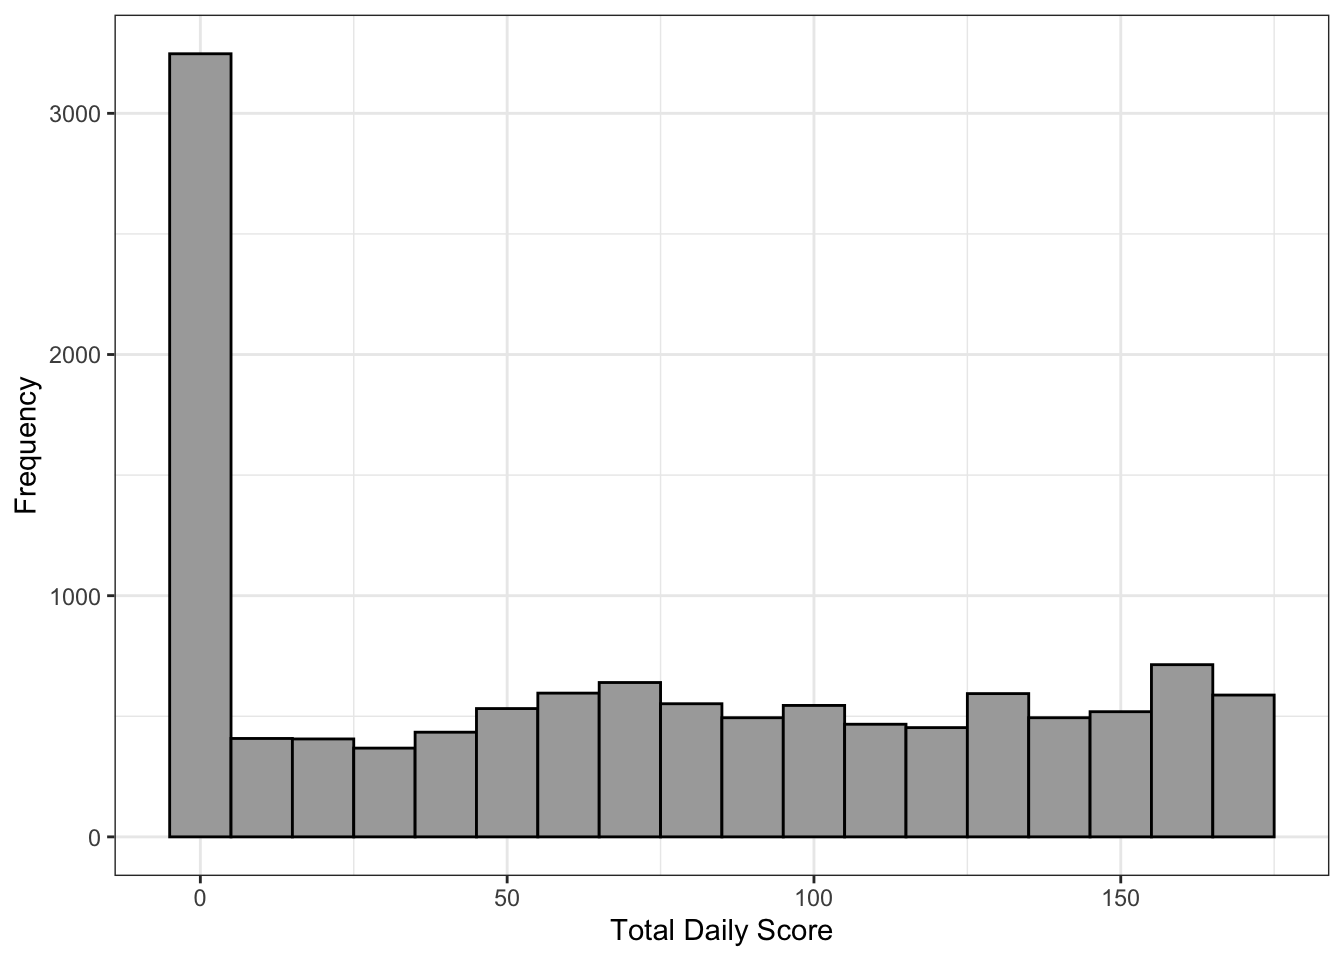
\includegraphics{03_methods_files/figure-pdf/fig-allScoredDays-1.pdf}

}

\caption{\label{fig-allScoredDays}Distribution of scores for all
userID-activity days.}

\end{figure}%

To understand what different quality LBS data days look like, we plotted
the number of LBS points for four random userID-activity days for each
hour to visualize the quality of the LBS data. These examples are shown
in Figure~\ref{fig-exampScoredDays}. The visualization of the number of
LBS points per hour, coupled with the score from the algorithm, offers a
beneficial insight into the data quality assessment. These randomly
chosen days serve as representative examples, showcasing the spectrum of
data quality inherent in our LBS dataset.

\begin{figure}[H]

\centering{

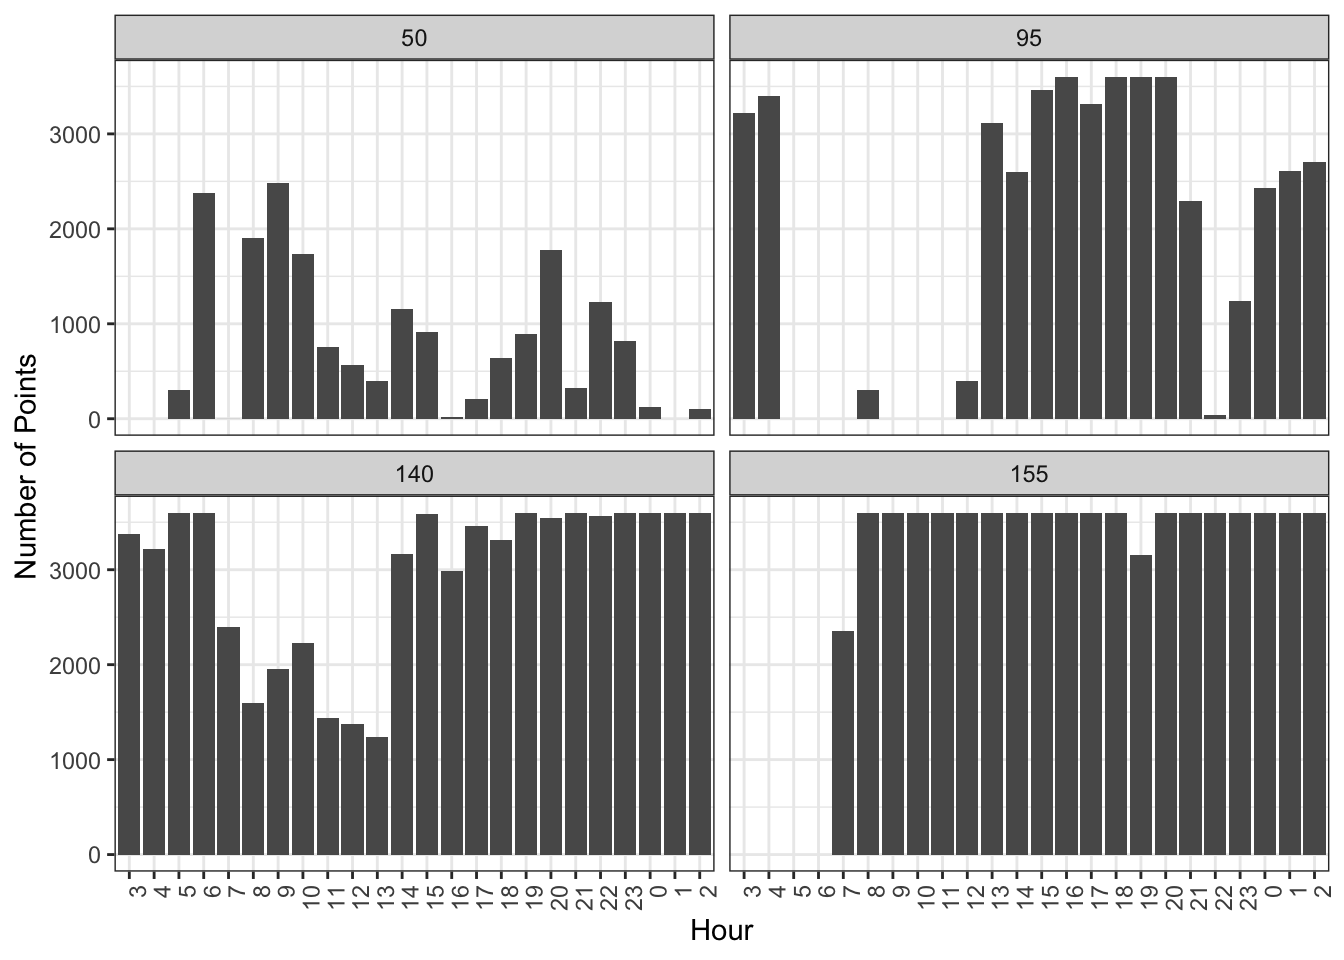
\includegraphics{03_methods_files/figure-pdf/fig-exampScoredDays-1.pdf}

}

\caption{\label{fig-exampScoredDays}Examples of daily LBS data for
differently scored userID-activity days.}

\end{figure}%

Once we determined the activity day and which userID-activity days had
high scores, indicating high quality and completeness, we trimmed down
some of the redundant LBS data. When the participants' phones were
turned on, the data collection application recorded an LBS data point
every second. To improve workability of the data and reduce the
redundancy of the LBS data points, we extracted a random sample of 6 LBS
points per minute for each high scoring userID-activity day. The same
sized random sample of LBS points was used in the optimization of the
DBSCAN-TE algorithm, which will be described in the following section
(Macfarlane et al., 2024).

All in all, the data cleaning process involved several crucial steps to
ensure the quality and integrity of the dataset. Initially, by shifting
the 24-hour period to be from 3:00 AM to 2:59 AM, we captured
individuals' daily travel more accurately, considering activities that
occurred after midnight but before 3:00 AM. This adjustment also aligned
with the closure of the evening mental health survey at 3:00 AM,
ensuring consistent association with the correct activity day.
Subsequently, we implemented a scoring algorithm to assess the quality
and completeness of the LBS data for each userID-activity day
combination. High scoring days, defined by a final score of 95 points or
more, were retained for further analysis, ensuring the inclusion of data
with sufficient completeness and accuracy. The scoring algorithm reduced
the number of user-ID activities days by 63\%. This selection process
resulted in a refined dataset ready for subsequent analysis.
Furthermore, to streamline the dataset and reduce redundancy, a random
sample of 6 LBS points per minute was extracted for each high scoring
userID-activity day. These steps collectively ensured that the dataset
was prepared for analyzing individual travel behavior and its
relationship with mental health outcomes.

\subsection{Processing the Data}\label{processing-the-data}

After preparing the data, we had a total of 4,405 userID-activity days
with sufficient data to implement the DBCAN-TE algorithm to determine
activity locations. The DBSCAN-TE algorithm classifies activities that
occurred during one's day. When given a set of points in some space, the
algorithm groups together points that are closely packed into clusters
and labels that cluster location as an activity. There are four
parameters in the DBSCAN-TE algorithm.

The first parameter is the epsilon neighborhood distance, \(\epsilon\),
which defines the radius within which points must fall to be considered
part of a cluster. The second parameter is the minimum number of points,
\(\rho\), representing the minimum number of points that must be present
within the defined radius for it to be considered a cluster.
Figure~\ref{fig-parameters_1_2} shows an example of the epsilon
neighborhood distance and minimum number of points.

\begin{figure}[H]

\centering{

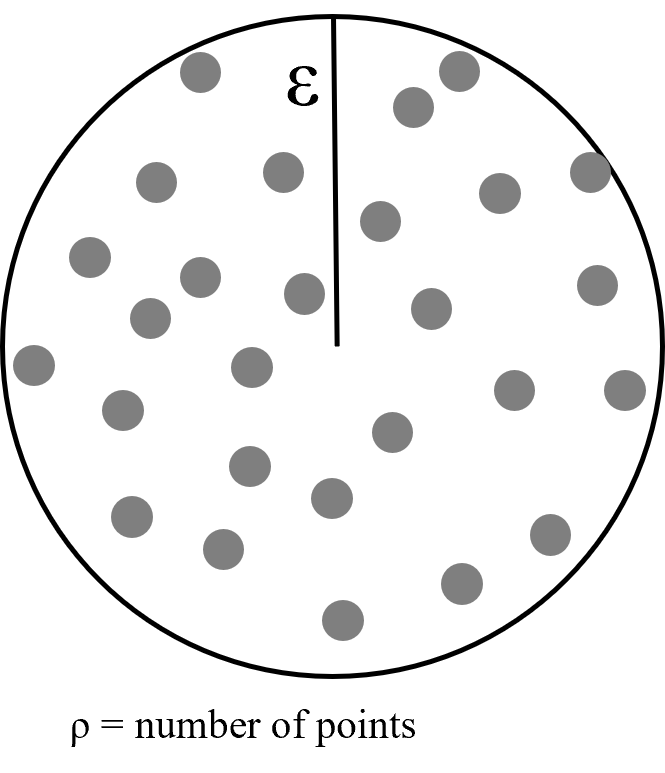
\includegraphics[width=2.5in,height=\textheight]{parameters_1_2.png}

}

\caption{\label{fig-parameters_1_2}DBSCAN-TE: Epsilon neighborhood
distance and minimum number of points.}

\end{figure}%

The temporal sequence constraint, \(\Delta T\), which is the third
parameter, ensures that clusters do not include points with a
significant gap in timestamps. \(\Delta T\) is the maximum time interval
allowed between two consecutive points in a cluster before it is
considered that multiple activities occurred within the same cluster at
different times. This is achieved by calculating the time difference
between each consecutive point in the spatial cluster. If the time
elapsed between any two consecutive points within the cluster exceeds
the \(\Delta T\) constraint, the cluster is divided into two at that
point. For instance, if the data points in cluster 1.0 exceed the
\(\Delta T\) constraint, the cluster would be split into two: 1.0 and
1.1. This concept for hypothetical consecutive points 1 through 7 is
illustrated in Figure~\ref{fig-parameter_3}. For example, LBS points
from 8:00 AM and 9:00 PM should not belong to the same cluster if there
are intervening points from another location. In this situation, the LBS
points would be split into separate clusters, assuming the individual
left and later returned to the activity location.

\begin{figure}[H]

\centering{

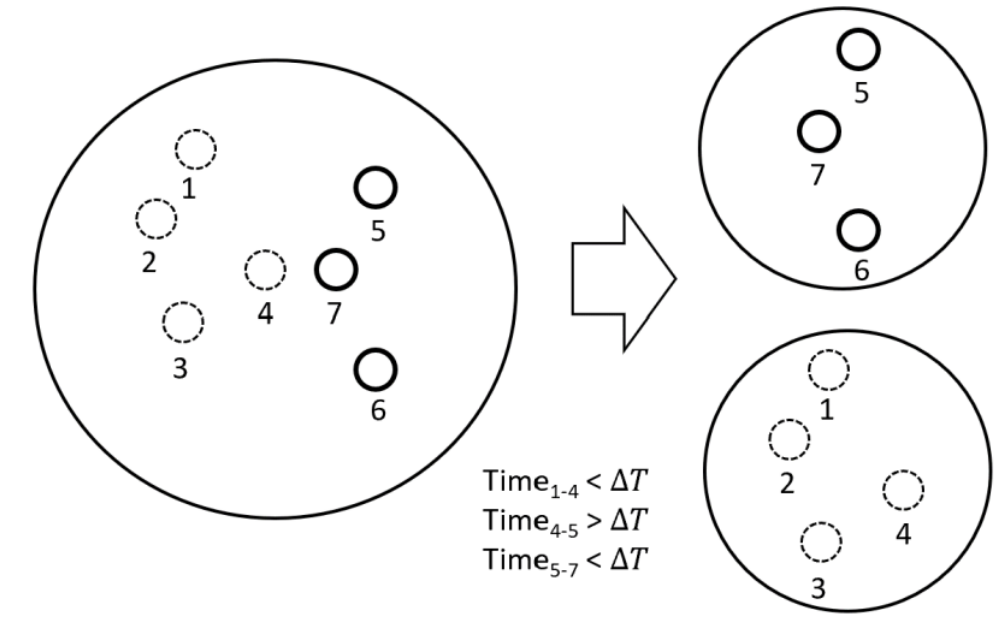
\includegraphics[width=5in,height=\textheight]{parameter_3.png}

}

\caption{\label{fig-parameter_3}DBSCAN-TE: Temporal sequence
constraint.}

\end{figure}%

The fourth parameter is the entropy constraint, \(\tau\), which
determines whether LBS points are part of a stationary cluster or a
moving trajectory. This parameter prevents slowly moving points from
being misidentified as clusters by examining the chaos and pattern of
LBS data. For example, points moving slowly in an orderly pattern, such
as driving from stoplight to stoplight, are excluded. However, slowly
moving but sporadic points, indicating movement within a single location
like a building or park, can be part of a cluster.

The entropy of each cluster is calculated by determining the distance
and angle in radians between consecutive points. The distance of a ray
represents the time elapsed between two consecutive points, while the
angle indicates the direction of movement. All the rays in the cluster
are plotted within a 2π circle divided into 8 quadrants. If multiple
rays from the same cluster fall within the same quadrant, they are
considered orderly and likely represent a moving trajectory rather than
a stationary cluster. Conversely, if the rays are distributed across
different quadrants, they are considered chaotic and more likely to
indicate a cluster or activity. Examples of hypothetical consecutive
points 1 through 7 with low and high entropy are shown in
Figure~\ref{fig-parameter_4}.

\begin{figure}[H]

\centering{

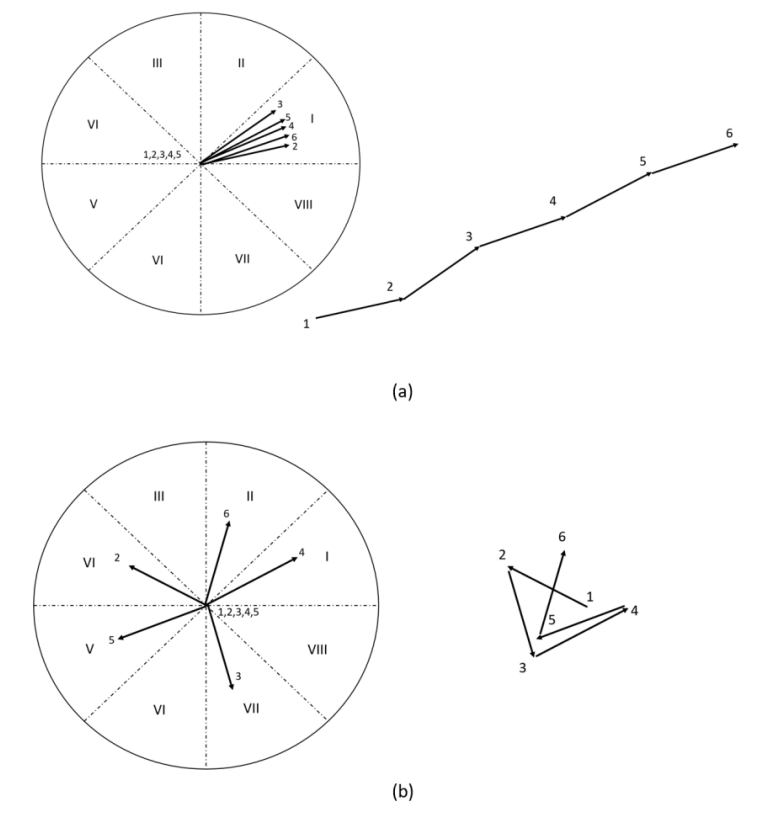
\includegraphics[width=5.5in,height=\textheight]{parameter_4.png}

}

\caption{\label{fig-parameter_4}DBSCAN-TE: Entropy constraint with (a)
low and (b) high entropy.}

\end{figure}%

These four parameters for the DBSCAN-TE algorithm were previously
optimized and applied to the LBS data to determine the activity
locations for each userID-activity day (Macfarlane et al., 2024).
Although the DBSCAN-TE algorithm was only used on high-scoring
userID-activity days, it did not produce results for all of them. Out of
the 4,405 userID-activity days, 3,845 yielded results after the
algorithm was implemented.

After identifying all the activity locations, we totaled them to
calculate the number of activities for each userID-activity day.
Figure~\ref{fig-numAct} shows the distribution of the number of
activities for the 3,845 userID-activity days. The average number of
activities engaged in each day was 2.65 activities.

\begin{figure}[H]

\centering{

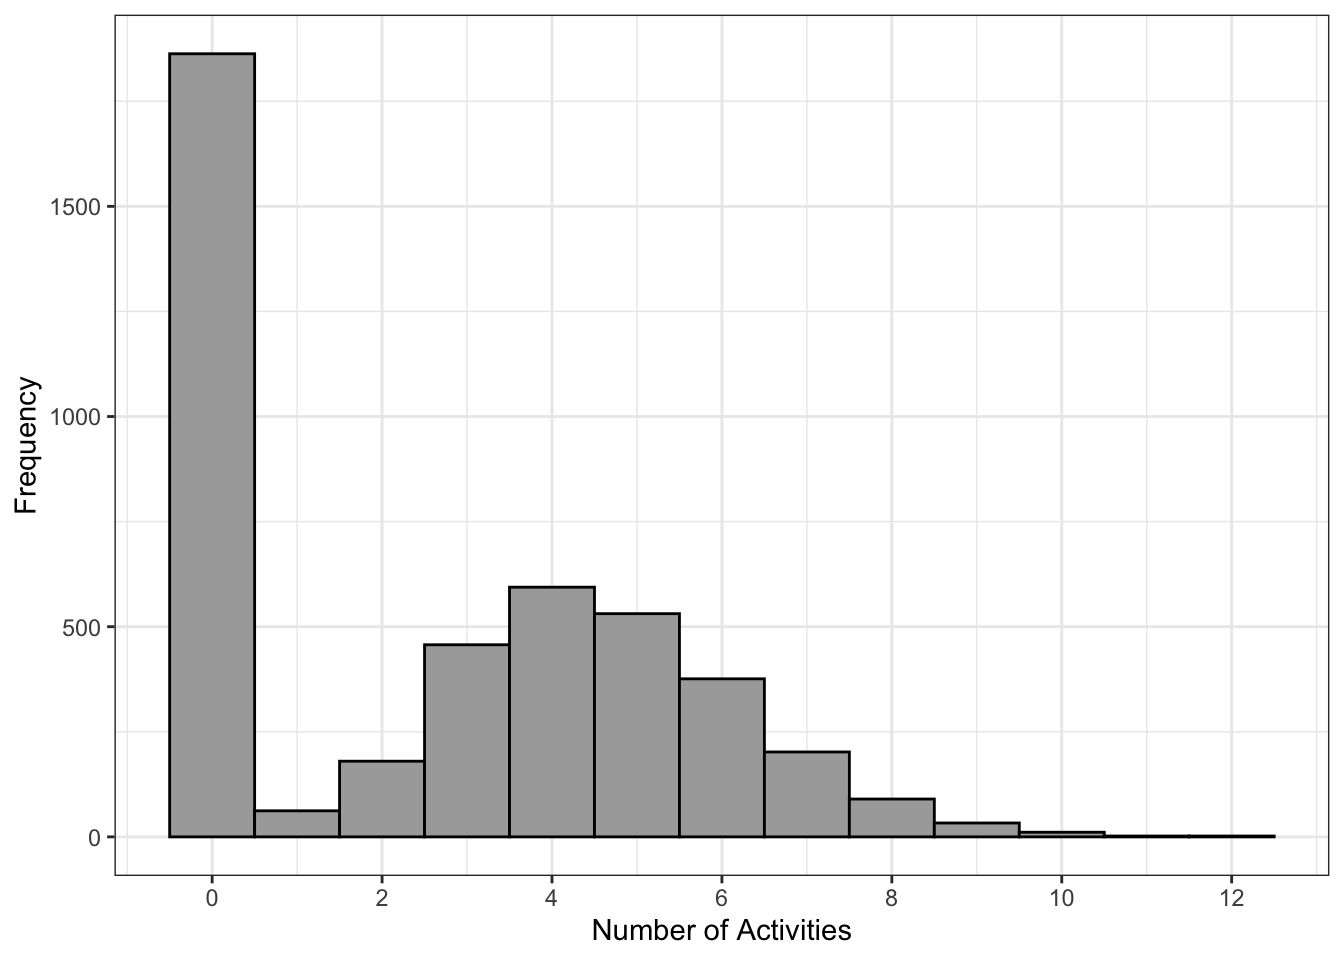
\includegraphics{03_methods_files/figure-pdf/fig-numAct-1.pdf}

}

\caption{\label{fig-numAct}Distribution of activities per day for all
userID-activity days.}

\end{figure}%

As many participants participated in the study over multiple months, the
DBSCAN-TE algorithm identified activities across various regions of the
United States. Since all of the participants reside in Utah County,
Utah, the majority of the activities are clustered within Utah County.
To visually represent the distribution of activities,
Figure~\ref{fig-actLocs} illustrates all identified activities within
this geographical area. Notably, a significant concentration of activity
points emerges in Provo, close to BYU campus, a pattern consistent with
expectations since the study was conducted by the BYU CAPS office.

\begin{verbatim}

  |                                                                            
  |                                                                      |   0%
  |                                                                            
  |==================                                                    |  25%
  |                                                                            
  |===================================                                   |  50%
  |                                                                            
  |====================================================                  |  75%
  |                                                                            
  |======================================================================| 100%
\end{verbatim}

\begin{figure}[H]

\centering{

\includegraphics{03_methods_files/figure-pdf/fig-actLocs-1.pdf}

}

\caption{\label{fig-actLocs}Activity locations for all userID-activity
days in Utah County.}

\end{figure}%

In addition to determining the total number of activities for each
userID-activity day, we also determined the number of activities that
took place at four specific location types. To do this, we used
OpenStreetMap data to create GeoJSON shapefiles for the locations of
parks, grocery stores, libraries, and social recreation sites in Utah
County. Then, we overlaid the spatial geometry of the activities with
the GeoJSON shapefiles to determine the number of activities that
occurred at the specific locations types.

After determining the total number of activities and their respective
types, an imputation procedure was executed to enhance dataset
completeness. This process aimed to address missing activity data on
certain days, whether due to data collection absence or data quality
issues, ensuring better alignment with completed mental health surveys.
Using rolling averages, missing activity data was estimated for specific
timeframes over varying time windows (seven, 14, and 30 days) to capture
activity trends. The imputation process was applied to total activities
and separately for distinct activity types (e.g., parks, grocery stores,
libraries, social recreation locations) to accommodate potential
variations in activity patterns across contexts.

After applying the rolling averages, we found that there were 5,673
userID-activity days for the seven-day rolling average, 6,252
userID-activity days for the 14-day rolling average, and 7,130
userID-activity days for the 30-day rolling average.

Figure~\ref{fig-numActsev} show the distribution of activities for the
seven-day rolling average, as an example.

\begin{figure}[H]

\centering{

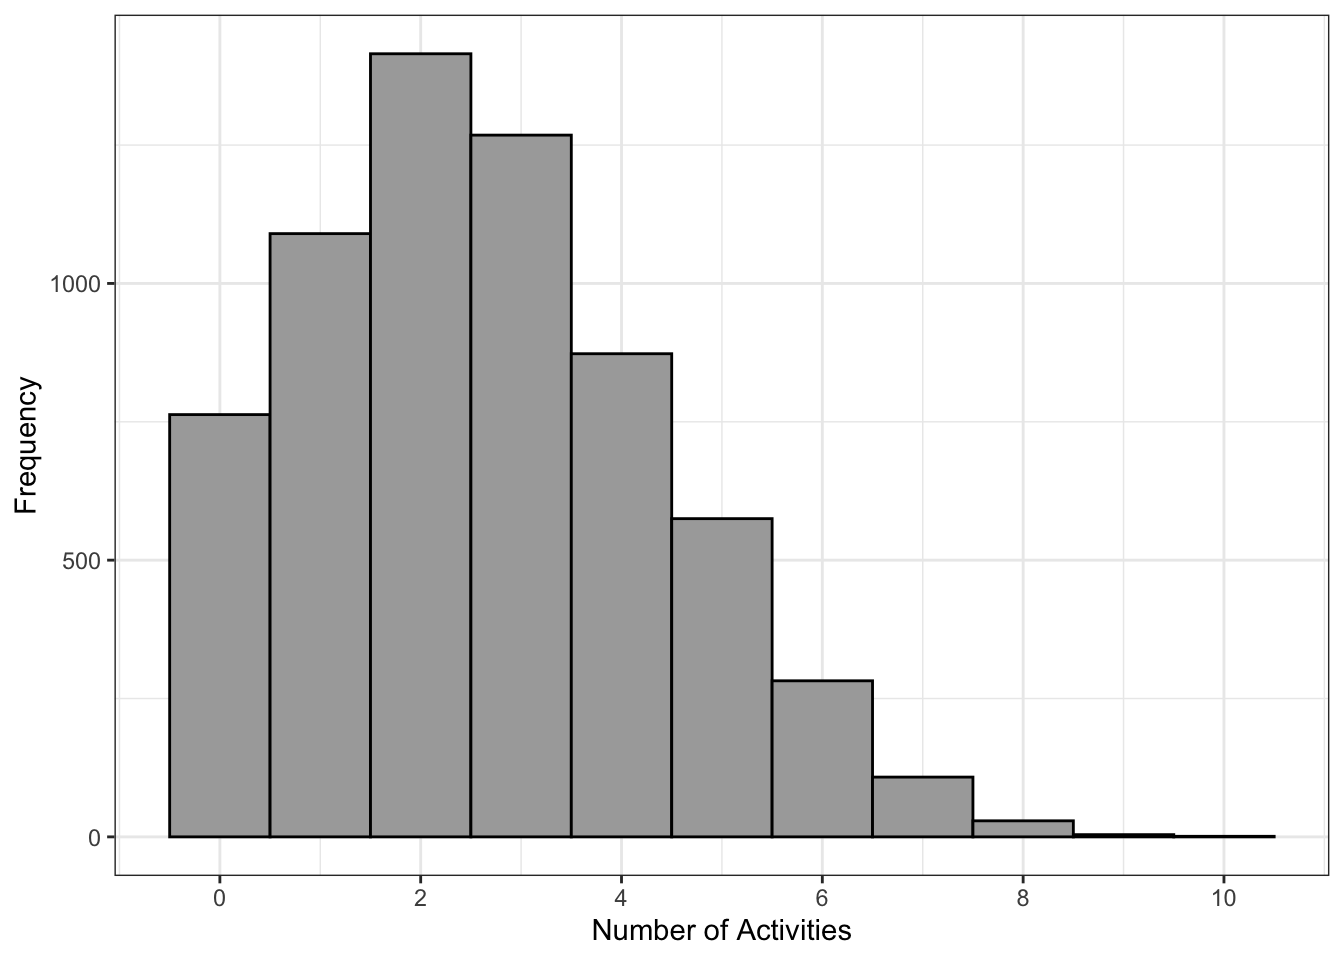
\includegraphics{03_methods_files/figure-pdf/fig-numActsev-1.pdf}

}

\caption{\label{fig-numActsev}Distribution of seven-day rolling average
number of activities for all userID-activity days.}

\end{figure}%

By calculating rolling averages and imputing missing activity data, the
imputation algorithm enhanced the dataset's completeness and
reliability, thereby facilitating more robust analyses of activity
patterns and their associations with mental health outcomes.

\subsection{Additional Travel
Parameters}\label{additional-travel-parameters}

In addition to analyzing the number of activities and their locations,
we analyzed other parameters to describe the travel patterns of
individuals. These parameters were included because while the accuracy
of the DBSCAN-TE algorithm in identifying activities is 91.5\% accurate,
it is not 100\% accurate (Riches, 2022). We noticed some inaccuracy when
we examined some of the raw LBS data. Instances appeared where
activities seemed apparent but went undetected by the algorithm. These
discrepancies prompted a deeper investigation into additional parameters
that might shed light on daily travel patterns.

The additional parameters we introduced were the convex hull area and
total distance traveled. The convex hull is the shape formed by
connecting the outermost points of the LBS points in such a way that the
resulting polygon is convex, meaning that any line segment connecting
two points within the shapes lies entirely within the shape itself. By
calculating the area enclosed by the convex hull, we gained a measure of
the geographic footprint of the recorded LBS data, independent of the
location of activities. This value is reported in square kilometers.
Figure~\ref{fig-convex_hull_area} illustrates the convex hull of a set
of hypothetical LBS points.

\begin{figure}[H]

\begin{minipage}{0.05\linewidth}
~\end{minipage}%
%
\begin{minipage}{0.40\linewidth}

\centering{

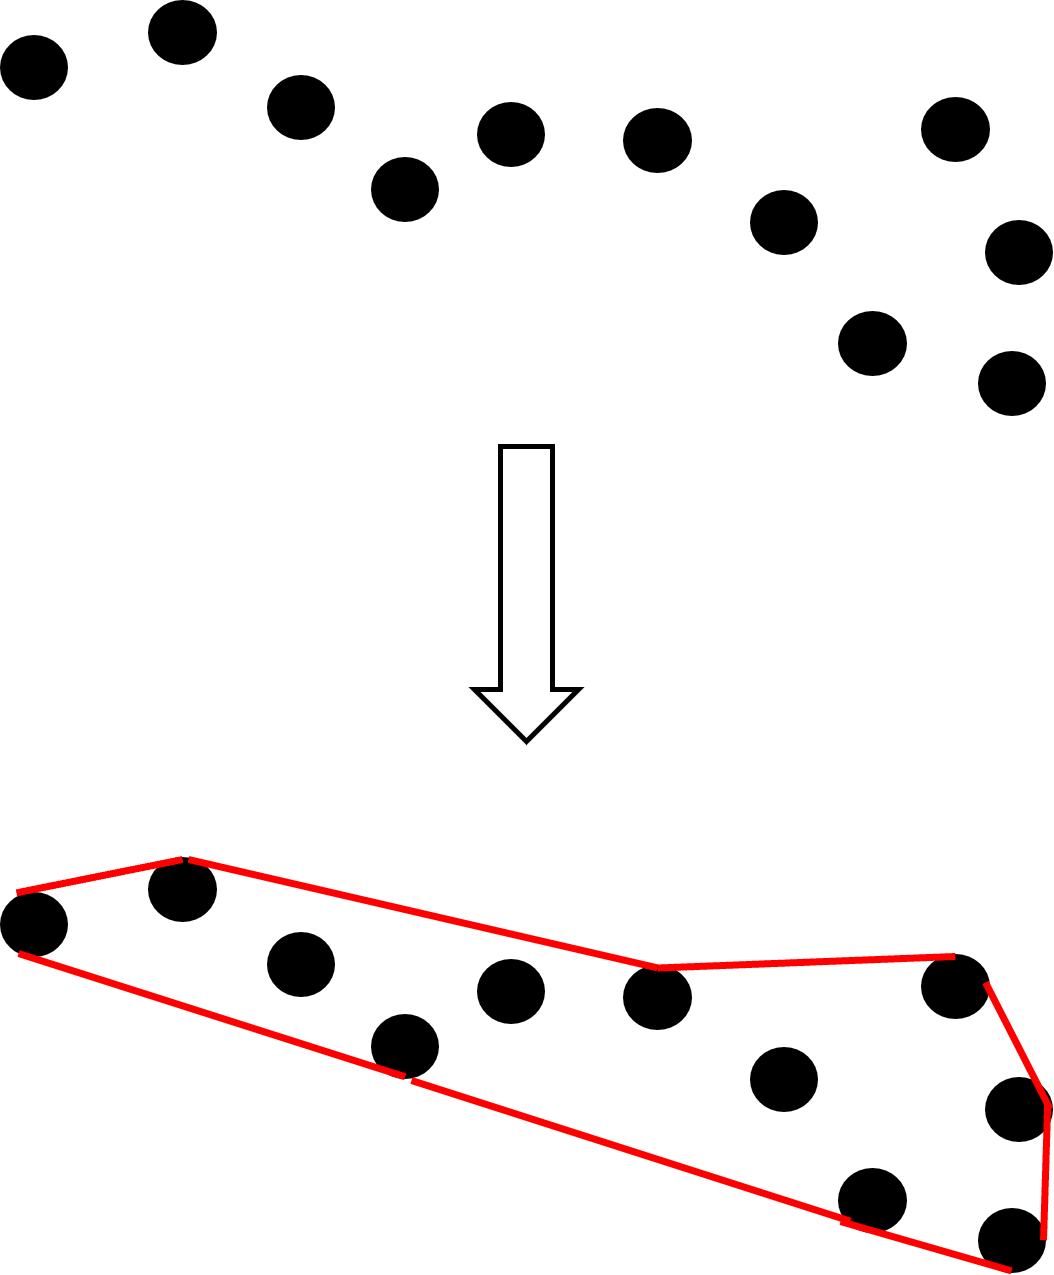
\includegraphics{convex_hull_area.png}

}

\subcaption{\label{fig-convex_hull_area}Convex hull area}

\end{minipage}%
%
\begin{minipage}{0.10\linewidth}
~\end{minipage}%
%
\begin{minipage}{0.40\linewidth}

\centering{

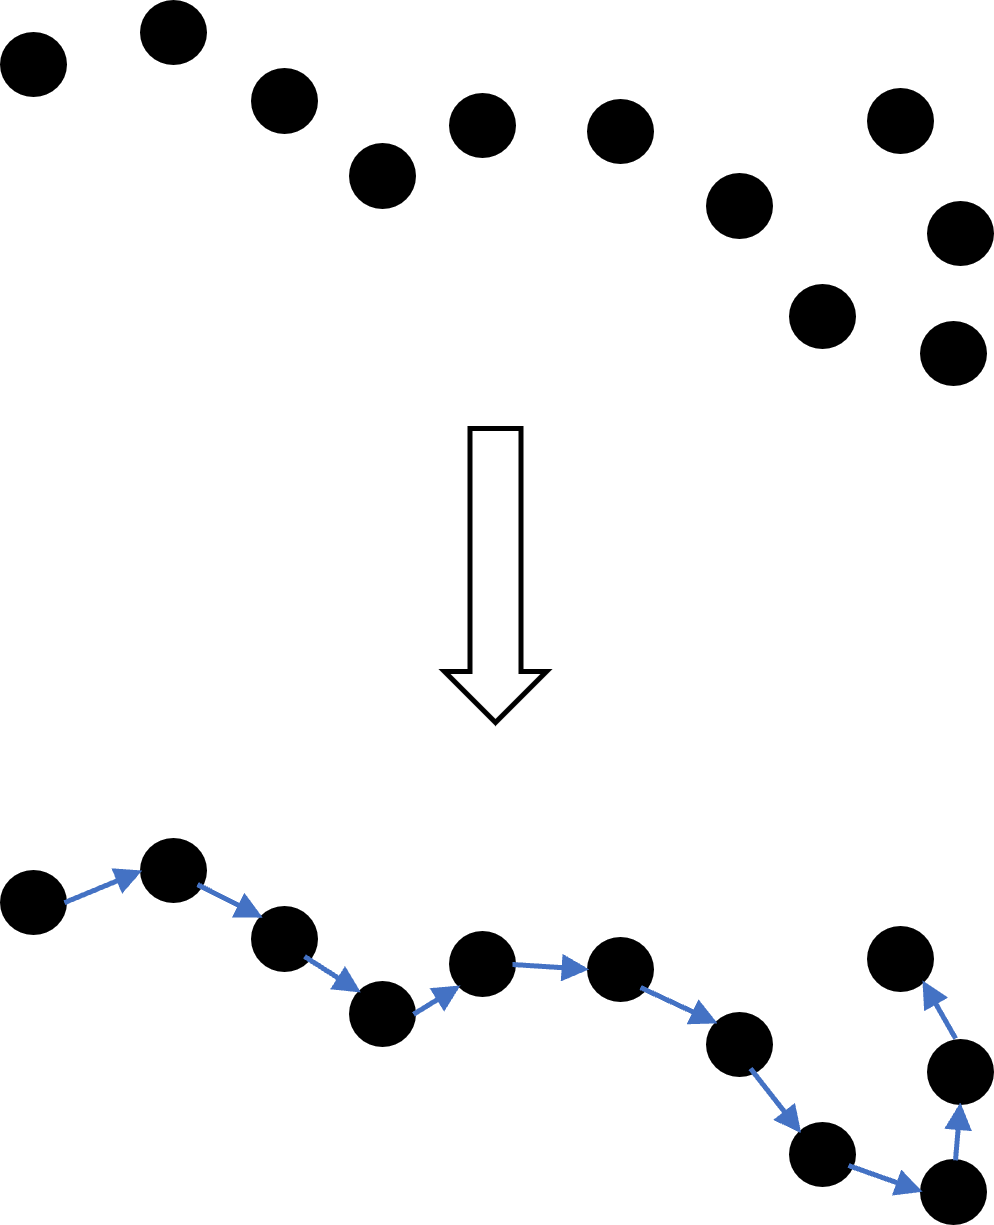
\includegraphics{distance_travelled.png}

}

\subcaption{\label{fig-distance_travelled}Total distance traveled}

\end{minipage}%
%
\begin{minipage}{0.05\linewidth}
~\end{minipage}%

\caption{\label{fig-travel_params}Additional travel parameters.}

\end{figure}%

We also evaluated the total distance traveled by each individual on each
activity day. To determine the total distance traveled, we computed the
length of the polyline, representing the trajectory of movement between
consecutive LBS points, during a participant's day. This value is
reported in meters. Figure~\ref{fig-distance_travelled} illustrates the
total distance traveled of a set of hypothetical LBS points.

Overall, our analysis more than merely quantified the number of
activities and their locations as we introduced two additional
parameters, the convex hull area and total distance traveled, to
contribute to a comprehensive characterization of travel patterns.

\subsection{Completed Processing of the LBS
Data}\label{completed-processing-of-the-lbs-data}

With the data carefully prepared, processed into distinct activity
categories and locations, and supplemented with additional parameters,
we laid a foundation for exploring the relationship between travel
behavior and mental well-being. These comprehensive insights including
parameters like convex hull area and total distance traveled, now allow
us to explore how individual travel patterns intertwine with responses
to mental health surveys. By scrutinizing the interplay between travel
behavior and activity engagement alongside mental health outcomes, our
analysis looks to find nuanced connections that can inform and foster
holistic well-being for individuals in different groups.

\subsection{Statistical Modeling}\label{statistical-modeling}

We combined semantic activities, travel pattern parameters, and survey
responses to create statistical models that explore the relationship
between mental health and travel behavior. Using motivation as an
indicator of overall mental health and well-being, we analyzed how
various factors influenced motivation, as represented in
Equation~\ref{eq-motivation}
\begin{equation}\phantomsection\label{eq-motivation}{
\text{Motivation}_{it} \; \tilde{} \; \beta (\vec{X}_{it})
}\end{equation}

We examined a range of models using various variables related to the
individuals and their travel behavior. These variables are outlined in
Equation~\ref{eq-variables}
\begin{equation}\phantomsection\label{eq-variables}{
X = 
\begin{cases} 
\text{individual descriptors}_i \\
\text{number of activities}_{it} \\
\text{avg. number of activities}_{i(t-t_7)} \\
\text{activity locations}_{it} \\
\end{cases}
}\end{equation}

For our analysis, we analyzed an ordinary least squares (OLS) model,
fixed effects (FE) model, and random effects (RE) model to determine
which was the best fit for our data (Wooldridge, 2009). For all three
models, the motivation, as reported in the evening surveys on a scale
from 0-100, served as the dependent variable. Participants used a drag
bar to indicate their motivation on the evening survey, with prompts
provided: ``0-19 None at all or little motivation'', ``20-39 Enough
motivation to get by'', ``40-59 Typical motivation'', ``60-79 Plenty of
motivation'', and ``80-100 Unusually high motivation feeling hyper or
even agitated at times''. The level of motivation was used as a measure
for overall well-being. Additionally, the seven-day rolling average
number of activities, as described previously, served as the independent
variable for the models. In addition to the model analysis, we accounted
for the potential for heteroskedasticity and autocorrelation in the
selected models.

\subsubsection{Ordinary Least Squares}\label{ordinary-least-squares}

Daily motivation levels were considered as a function of the seven-day
rolling average number of activities described in the previous sections.
Using these parameters, a linear regression model was estimated by OLS.
Equation~\ref{eq-ols} shows the base OLS equation where \(\alpha_{i}\)
represents the fixed effects in the model, or the time invariant
variables \begin{equation}\phantomsection\label{eq-ols}{
\text{Motivation} = \alpha_{i} + \beta (\text{sev-day avg. no. of acts.}_{it}) + \mu_{it}
}\end{equation} For linear regressions, it is assumed that the error
terms are independently and identically distributed (IID) with a normal
distribution of mean 0. The estimates resulting from this model may be
inconsistent due to unobserved individual differences (violating the IID
assumption). For example, all individuals have a different baseline or
typical level of motivation. We want to account for changes in
motivation by individual to see how their motivation deviates from its
baseline. There are two common econometric techniques, known as FE and
RE, that attempt to account for these baseline measures, which are
discussed in the following sections.

\subsubsection{Fixed Effects}\label{fixed-effects}

The FE model, also called the within transformation, demeans the data by
participant and looks at each participant's levels of motivation and
seven-day rolling average number of activities individually. This
results in having different intercepts for each participant.
Equation~\ref{eq-fe} shows the base equation for the FE model
\begin{equation}\phantomsection\label{eq-fe}{
y_{it} - \bar{y}_i = \beta ( x_{it} - \bar{x}_i ) + \mu_{it} -\bar{\mu}_i 
}\end{equation} Since \(\alpha_i\) from the OLS model is fixed overtime,
these unobserved effects disappear in the FE model. In this case, the
time constant characteristics are the demographic characteristics of
each participant. These variables are absorbed by the intercept as they
are unique to each participant.

The FE model is consistent but less efficient because it results in
losing degrees of freedom to estimate individual intercepts for each
participant. This results in larger standard errors for the estimates
which can make it more difficult to recognize significance.

\subsubsection{Random Effects}\label{random-effects}

The RE model semi-demeans the data by participant. Based on a mean for
the entire group, a mean is determined with a set standard deviation to
represent the data of the entire group. The RE model assumes that
\(\alpha_i\), the unobserved effect, is uncorrelated with the seven-day
rolling average number of activities. \(\lambda\) represents a
``transformation that eliminates serial correlation in the errors''
(Wooldridge, 2009, pg. 490). Equation~\ref{eq-re} shows the base
equation for the RE model \begin{equation}\phantomsection\label{eq-re}{ 
y_{it}-\lambda\bar{y}_i = \beta_0(1-\lambda)+\beta_1 ( x_{it1}-\lambda\bar{x}_{i1})+...+\beta_k (x_{itk}-\lambda\bar{x}_{ik})+(\nu_{it}-\lambda\bar{\nu}_i) 
}\end{equation}

\hfill\break
The RE model is appropriate to use if it is believed that the difference
in motivation has an influence on the seven-day rolling average number
of activities. It is possible that other variables that influence the
seven-day rolling average number of activities are not included which
can lead to bias in the model. Unlike the FE model, the RE model is more
efficient because degrees of freedom are not lost to more estimates, but
the results can be biased.

\subsubsection{Autocorrelation and
Heteroskedasticity}\label{autocorrelation-and-heteroskedasticity}

When analyzing how motivation changes over time for individual people,
autocorrelation and heteroskedasticity can arise as statistical
challenges. Autocorrelation occurs when observations in a time series
are correlated with preceding or succeeding observations, violating the
assumption of independence between observations. In the context of
studying individual motivation over time, autocorrelation can manifest
as a person's motivation level at one point in time being influenced by
their motivation level at previous time points. This can lead to biased
estimates and inflated significance levels in regression analyses.
Heteroskedasticity refers to the unequal variance of errors across
observations in a dataset. In the case of studying motivation over time,
heteroskedasticity may arise if the variability in motivation levels
differs between individuals or varies systematically over time. This
violates the assumption of homoscedasticity, where the variance of the
errors remains constant across observations.

Autocorrelation and heteroskedasticity can lead to biased parameter
estimates or incorrect inference in statistical models. To address these
issues, robust measures for standard errors are used. Specifically in
our case, Heteroskedasticity and Autocorrelation Consistent (HAC)
standard errors can be employed. HAC robust standard errors are
particularly useful when dealing with time series or panel data where
observations may be correlated across time periods. HAC estimators
adjust for heteroskedasticity by allowing the variance of the errors to
vary across observations. However, they also account for autocorrelation
by incorporating a weighting scheme that considers the correlation
structure of the data over time. This weighting scheme assigns higher
weights to more recent observations and lower weights to distant
observations, reflecting the diminishing influence of past observations
on current ones.

By adjusting for both heteroskedasticity and autocorrelation, HAC robust
standard errors provide more accurate estimates of the standard errors
of regression coefficients, ensuring valid statistical inference in the
presence of correlated and heteroskedastic data.

\bookmarksetup{startatroot}

\section{Results and Discussions}\label{results-and-discussions}

Analyzing travel behavior and mental well-being requires a comprehensive
examination of the individual's group. It is important to look at
various factors related to how these groups travel and how their travel
affects their well-being. Understanding the number and type of
activities they engage in, motivational levels, and propensity towards
suicidal ideation provides valuable insights for this analysis.

\subsection{Activity Engagement by
Group}\label{activity-engagement-by-group}

This analysis examined the activity engagement patterns of the three
groups: control, autism, and social anxiety. We analyzed the total
number of activities and the seven-day rolling average number of
activities for individuals in these groups. The descriptive statistics
in Table~\ref{tbl-groupActs} describe these results for each group.

\begin{table}

\caption{\label{tbl-groupActs}Activity Descriptive Statistics by Group}

\centering{

\centering
\resizebox{\linewidth}{!}{
\begin{tabular}[t]{lcccccc}
\toprule
\multicolumn{1}{c}{ } & \multicolumn{2}{c}{Control (N=1706)} & \multicolumn{2}{c}{Autism (N=804)} & \multicolumn{2}{c}{Social Anxiety (N=1893)} \\
\cmidrule(l{3pt}r{3pt}){2-3} \cmidrule(l{3pt}r{3pt}){4-5} \cmidrule(l{3pt}r{3pt}){6-7}
  & Mean & Std. Dev. & Mean & Std. Dev. & Mean & Std. Dev.\\
\midrule
No. of Activities & 3.0 & 2.7 & 2.1 & 2.3 & 2.6 & 2.7\\
Sev-Day No. of Acts. & 3.0 & 1.7 & 2.0 & 1.4 & 2.6 & 1.7\\
\bottomrule
\end{tabular}}

}

\end{table}%

Starting with the total number of activities, individuals in the control
group had a moderate level of engagement, with an average number of 3.0
activities. In contrast, participants in the autism group had a lower
average number of activities, with a mean of 2.1 activities. Similarly,
individuals with social anxiety had a mean of 2.6 activities, falling
between the control and autism groups. The standard deviations for the
three groups ranged from 2.3-2.7. Moving to the seven-day rolling
average of activities, trends mirrored those of the total number of
activities, with slightly lower standard deviations, indicating less
variability in the rolling average compared to the total count.

To determine if significant differences existed in the mean number of
activities between the three groups, we conducted an ANOVA test. The
results unveiled a highly significant effect of the group on the number
of activities, as evidenced by an F value of 32.97 and a p-value less
than 0.001. This supports that the variation in the number of activities
across the groups was unlikely to be attributed to random chance,
confirming that there were significant differences among the groups.
Figure~\ref{fig-ANOVAActs} shows the mean number of activities and 95\%
confidence intervals for the differences between the corresponding group
means.

\begin{figure}[H]

\centering{

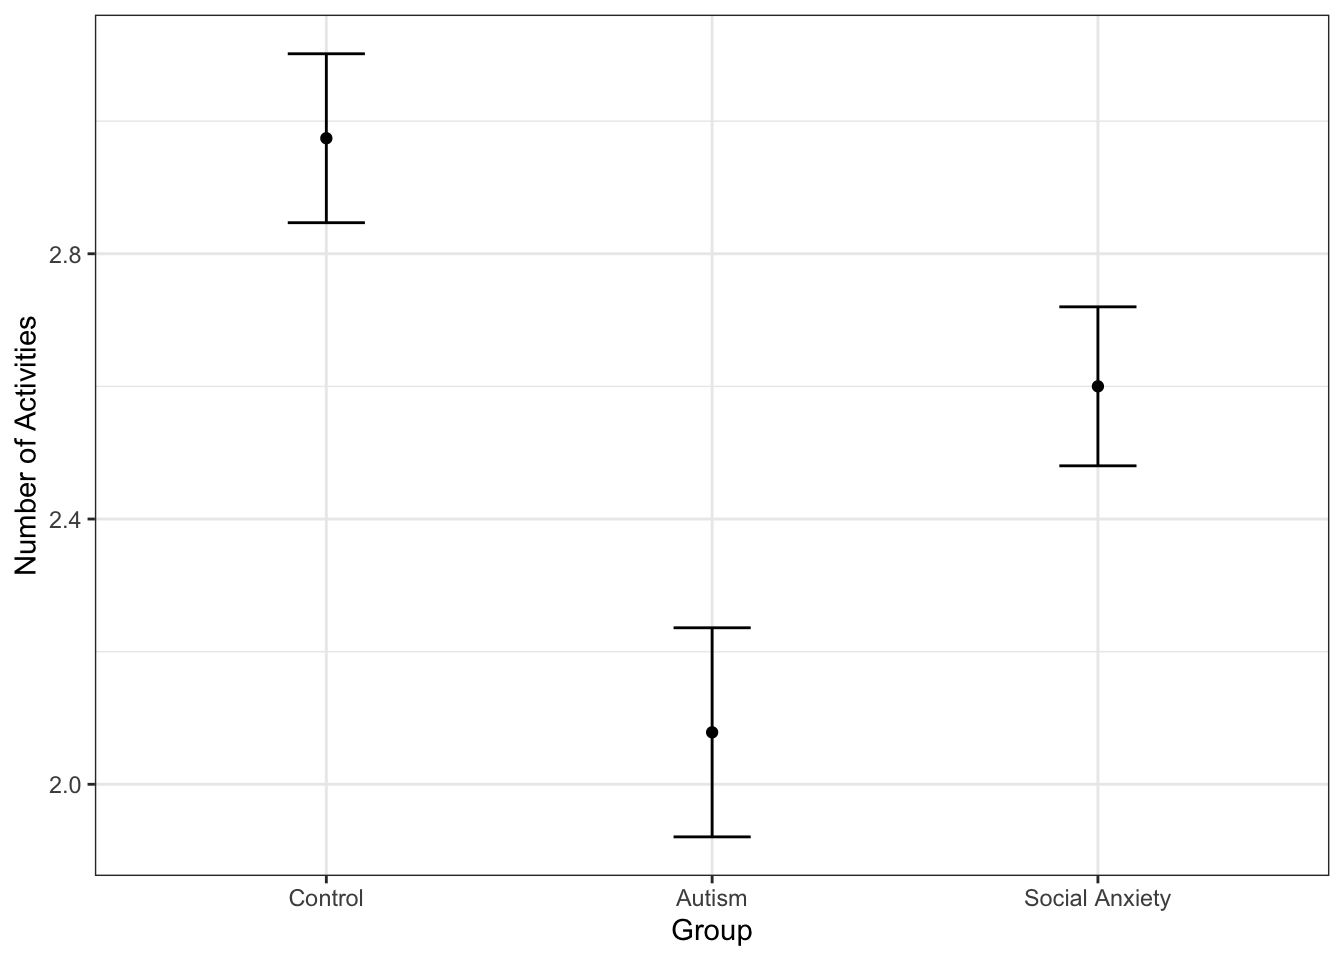
\includegraphics{04_results_files/figure-pdf/fig-ANOVAActs-1.pdf}

}

\caption{\label{fig-ANOVAActs}Mean number of activities by group.}

\end{figure}%

After we determined that there were significant differences in the mean
number of activities among three groups, a Tukey's Honest Significant
Difference (HSD) test was conducted to pinpoint which specific groups
differ from each other. Tukey's HSD test indicated that there were
significant differences in the mean number of activities between all
pairs of groups. Specifically, individuals in the autism group engaged
in significantly fewer activities on average compared to those in the
control group, with a mean difference of -0.896 and a p-value less than
0.001. Individuals in the autism group also engaged in significantly
fewer activities on average compared to those in the the social anxiety
group, with a mean difference of -0.375 and a p-value less than 0.001.
Similarly, participants in the social anxiety group participated in
significantly fewer activities on average than those in the control
group with a mean difference of -0.521 and a p-value less than 0.001.

These findings suggest that there are significant differences in the
mean number of activities among individuals belonging to the different
groups. Specifically, individuals with autism tend to engage in fewer
activities compared to both the control group and the social anxiety
group. Similarly, individuals in the social anxiety group participate in
fewer activities on average compared to those in the control group.
These results highlight the importance of considering group differences
when examining activity engagement patterns and potentially mental
health outcomes.

\subsection{Motivation by Group}\label{motivation-by-group}

Upon closer examination of the distinct groups, we noticed notable
differences in well-being. Based on the existing literature, we
anticipated that individuals in both the autism and social anxiety
groups would exhibit lower levels of well-being compared to those in the
control group. Given our use of motivation as an indicator of
well-being, we analyzed the reported levels of motivation across each
group, as reported in the evening survey on a scale from 1-100.
Table~\ref{tbl-groupMotiv} presents the mean and standard deviation of
motivation for each group.

\begin{table}

\caption{\label{tbl-groupMotiv}Motivation Levels by Group}

\centering{

\centering
\begin{tabular}[t]{lcccccc}
\toprule
\multicolumn{1}{c}{ } & \multicolumn{2}{c}{Control (N=1706)} & \multicolumn{2}{c}{Autism (N=804)} & \multicolumn{2}{c}{Social Anxiety (N=1893)} \\
\cmidrule(l{3pt}r{3pt}){2-3} \cmidrule(l{3pt}r{3pt}){4-5} \cmidrule(l{3pt}r{3pt}){6-7}
  & Mean & Std. Dev. & Mean & Std. Dev. & Mean & Std. Dev.\\
\midrule
Motivation & 47.7 & 14.2 & 34.0 & 19.4 & 40.3 & 18.5\\
\bottomrule
\end{tabular}

}

\end{table}%

The findings revealed differences in motivation levels across the
groups. The control group had the highest mean motivation score of 47.7,
falling slightly below the middle range of the ``typical motivation''
category, with the lowest standard deviation of 14.2. This suggests that
individuals in the control group generally have moderate motivation
levels with relatively little variability, indicating a consistent trend
of moderate motivation within this group. In contrast, the autism group
showed the lowest mean motivation score of 34.0, falling in the ``enough
motivation to get by'' category, with the highest standard deviation of
19.4. The lower mean score implied that individuals with autism tend to
have lower motivation levels compared to those in the control group. The
social anxiety group fell in the middle with a mean motivation score of
40.3, which is on the lowest end of the ``typical motivation'' category.

An ANOVA test was conducted to determine if there were significant
differences in the mean levels of motivation among the three groups. The
results revealed a highly significant effect of the group on motivation
levels, with an F value of 362 and a p-value less than 0.001. This
indicates that the variation in motivation levels across the groups is
unlikely to be due to random chance, and there are indeed significant
differences among the groups.

After determining that there significant differences in the mean levels
of motivation among the three groups, a Tukey's HSD test was conducted
to pinpoint which specific groups differ from each other. The autism
group had a significantly lower mean motivation level compared to the
control group, with a difference of -9.99 points. Similarly, the social
anxiety group had a significantly lower mean motivation level compared
to the control group, with a difference of -7.74 points. When comparing
the social anxiety group to the autism group, the social anxiety group
showed a significantly higher mean motivation level by 2.25 points. All
three pairs had p-values less than 0.001. \clearpage Overall, the
results of the ANOVA test and Tukey's HSD test indicate that there are
significant differences in mean motivation levels among the three
groups. Specifically, the control group had significantly higher levels
of motivation compared to both the autism and social anxiety groups.
Moreover, the autism group had significantly higher motivation levels
than the social anxiety group. This pattern underscores the impact that
the group has on an individual's motivation.

\subsection{Suicidal Ideation by
Group}\label{suicidal-ideation-by-group}

The morning and evening surveys included different questions pertaining
to suicidal ideation. Specifically, the evening survey asked
participants the following questions:

\begin{itemize}
\item
  Have you thought about killing yourself in the past 12 hours or since
  you last took a survey?
\item
  How intense was your desire to kill yourself since the last survey you
  completed (or over the past 12 hours, if you didn't complete the last
  survey)?
\item
  How strong was your intention to kill yourself by suicide since the
  last survey you completed (or over the past 12 hours, if you didn't
  complete the last survey)?
\item
  How strong was your ability to resist the urge to kill yourself since
  the last survey you completed (or over the past 12 hours, if you
  didn't complete the last survey)?
\end{itemize}

The dataset presents an insightful glimpse into the prevalence of
suicidal ideation within the groups, shedding light on potential
differences in mental health concerns among them. We examined responses
to the question ``Have you thought about killing yourself in the past 12
hours or since you last took a survey?'' across the three groups, where
responses were ``Yes,'' ``No,'' or ``No Response.'' The responses to
this question are summarized by group in Table~\ref{tbl-groupSuicide}.

\begin{table}

\caption{\label{tbl-groupSuicide}Suicidal Ideation by Group}

\centering{

\centering
\begin{tblr}[         %% tabularray outer open
]                     %% tabularray outer close
{                     %% tabularray inner open
colspec={Q[]Q[]Q[]Q[]Q[]Q[]Q[]Q[]},
cell{1}{3}={c=2,}{halign=c,},
cell{1}{5}={c=2,}{halign=c,},
cell{1}{7}={c=2,}{halign=c,},
column{1}={halign=l,},
column{2}={halign=l,},
column{3}={halign=c,},
column{4}={halign=c,},
column{5}={halign=c,},
column{6}={halign=c,},
column{7}={halign=c,},
column{8}={halign=c,},
row{1}={halign=c,},
}                     %% tabularray inner close
\toprule
&  & Control (N=1706) &  & Autism (N=804) &  & Social Anxiety (N=1893) &  \\ \cmidrule[lr]{3-4}\cmidrule[lr]{5-6}\cmidrule[lr]{7-8}
&    & N & Pct. & N & Pct. & N & Pct. \\ \midrule %% TinyTableHeader
Suicidal Ideation & Yes         & 36   & 2.1  & 39  & 4.9  & 296 & 15.6 \\
& No          & 1133 & 66.4 & 415 & 51.6 & 737 & 38.9 \\
& No Response & 537  & 31.5 & 350 & 43.5 & 860 & 45.4 \\
\bottomrule
\end{tblr}

}

\end{table}%

In the control group, on 66.4\% of days participants responded
negatively, indicating they did not think about killing themselves.
However, on 2.1\% of days, group members acknowledged experiencing
suicidal ideation during the specified timeframe. Contrastingly, among
respondents with autism, on 51.6\% of the days, participants denied
having suicidal thoughts, while respondents admitted to suicidal
ideation with a slightly higher percentage on 4.9\% of days. In the
social anxiety group, the dynamics were notably different. Here,
participants reported no suicidal ideation on a significantly lower
percentage, 38.9\% of days, while they reported suicidal ideation on a
strikingly higher proportion of days, at 15.6\% of days. Across all
three groups, there was a portion of respondents who chose not to
provide a response, perhaps indicating the sensitivity of the question
or reluctance to disclose personal struggles.

To dive deeper into the suicidal ideation of individuals in the
different groups, we constructed a contingency table with the data
organized into rows and columns, with each row representing a group
(control, autism, and social anxiety) and each column representing a
response category (``Yes,'' ``No,'' or ``No Response'') regarding
suicidal ideation. Within the table, the counts of individual responses
in each group were recorded. Subsequently, a chi-square test of
independence was conducted on these counts to assess whether there is a
significant association between the group and the response to suicidal
ideation. The test calculated a chi-square statistic of 388.06 with 4
degrees of freedom. The resulting p-value was found to be less than
0.001, signifying substantial evidence against the null hypothesis of no
association. Thus, the analysis concluded that there is a statistically
significant association between the group and the response to suicidal
ideation. This suggests that the group typology influences the
likelihood of a particular response to suicidal ideation, indicating
potential differences in how individuals from different groups perceive
and experience suicidal ideation. These findings offer valuable insights
into the interplay between group and experience with suicidal ideation.

\subsection{Model Comparison and
Evaluation}\label{model-comparison-and-evaluation}

As discussed previously, we ran three different models to analyze the
effect of the seven-day rolling average number of activities on
motivation levels. We ran the OLS, FE, and RE models with robust
standard errors and t-statistics due to the potential for
autocorrelation and heteroskedasticity. The results of these three
models are shown in Table~\ref{tbl-olsfere}.

\begin{table}

\caption{\label{tbl-olsfere}OLS, FE, and RE Models}

\centering{

\centering
\begin{talltblr}[         %% tabularray outer open
entry=none,label=none,
note{}={Robust t-statistics in parentheses. + p < 0.1, * p < 0.05, ** p < 0.01, *** p < 0.001},
]                     %% tabularray outer close
{                     %% tabularray inner open
colspec={Q[]Q[]Q[]Q[]},
column{1}={halign=l,},
column{2}={halign=c,},
column{3}={halign=c,},
column{4}={halign=c,},
hline{4}={1,2,3,4}{solid, 0.05em, black},
}                     %% tabularray inner close
\toprule
& OLS & FE & RE \\ \midrule %% TinyTableHeader
Sev-Day No. of Acts. & 1.420*** & 0.287+    & 0.362*   \\
& (9.057)  & (1.691)   & (2.174)  \\
No. of Obs.          & 4,211    & 4,211     & 4,211    \\
AIC                  & 35,969.8 & 34,519.76 & 34,596.1 \\
R²                   & 0.021    & 0.001     & 0.047    \\
\bottomrule
\end{talltblr}

}

\end{table}%

\clearpage

We used the Hausman test to determine whether the RE model is more
appropriate than the FE model. The Hausman test tests whether the RE
estimates are consistent and efficient compared to the FE estimates. The
null hypothesis is that the RE estimates are consistent and efficient,
while the alternative hypothesis is that the FE estimates are more
efficient. We found, using the Hausman test, that the p-value is 0.0013
which is less than 0.05, which means that the results are significant
and we reject the null hypothesis. This implies that the coefficients
from the FE model and RE model are sufficiently different from each
other, which means that the RE model is inconsistent and the FE model
should be used for the remainder of the analysis.

\subsection{Effect of Demographic Factors on
Motivation}\label{effect-of-demographic-factors-on-motivation}

Based on the results of the Hausman test, we found that the FE model
should be used in the analysis of the activity pattern and mental health
data. One potential downside of the FE model is that it cannot implement
time constant variables. To overcome this limitation, we performed a
linear regression analysis to examine how demographic variables (e.g.,
sex, age, IQ score, and group) are associated with the intercepts from
the FE model. This linear regression is described generally in
Equation~\ref{eq-linreg}

\begin{equation}\phantomsection\label{eq-linreg}{
\bar{y}_{i} \; \tilde{} \; \beta (\vec{X}_{it})
}\end{equation}

This allows us to understand how the baseline levels of motivation
differ across groups. The sex, age, IQ score, and group were the
independent variables, and the FE intercept values for each userID
served as the dependent variable. The results from this model are shown
in Table~\ref{tbl-fedemolm}.

\begin{table}

\caption{\label{tbl-fedemolm}Fixed Effects and Demographics Regression}

\centering{

\centering
\begin{talltblr}[         %% tabularray outer open
entry=none,label=none,
note{}={t-statistics in parentheses. + p < 0.1, * p < 0.05, ** p < 0.01, *** p < 0.001},
]                     %% tabularray outer close
{                     %% tabularray inner open
colspec={Q[]Q[]},
column{1}={halign=l,},
column{2}={halign=c,},
hline{7}={1,2}{solid, 0.05em, black},
}                     %% tabularray inner close
\toprule
& Intercept Model \\ \midrule %% TinyTableHeader
Female         & -6.351 (-2.265)*   \\
Age            & 0.089 (0.192)      \\
IQ Score       & -0.058 (-0.617)    \\
Autism         & -10.247 (-3.139)** \\
Social Anxiety & -8.544 (-3.164)**  \\
No. of Obs.    & 62                 \\
Log. Liklihood & -222.022           \\
AIC            & 458.044            \\
R²             & 0.264              \\
\bottomrule
\end{talltblr}

}

\end{table}%

The analysis revealed several significant findings. First, being female
was associated with a decrease in motivation by 6.351 points, on a scale
from 0-100, compared to males, which is a statistically significant
effect with a p-values less than 0.05. Age and IQ score did not show
significant associations with motivation. Conversely, individuals with
autism exhibited a substantial decrease in motivation by 10.247 points
compared to the control group, and those with social anxiety experienced
a similar decrease of 8.544 points, both statistically significant
results with p-values less than 0.01. These results suggest that sex and
group status play significant roles in shaping motivational levels,
while age and IQ score appear to have limited influence in this context.
When looking at the fit of this model to the data, the model explains
approximately 26.4\% of the variance in motivation, indicating that
other unexplored factors may contribute to motivational outcomes. These
findings underscore the importance of considering individual
differences, particularly sex and group status, when examining levels of
motivation. For this analysis, the group typology is a main focus and
will continue to be explored.

\subsection{Model Comparison for Impact on
Motivation}\label{model-comparison-for-impact-on-motivation}

To compare the effects of different aspects of travel behavior on
motivation, we conducted a comprehensive analysis considering various
factors. Specifically, we examined the impact of the total number of
activities, the seven-day rolling average number of activities, the
convex hull area, and the total distance traveled on a day. Analyzing
the total number of activities provides insights into the overall level
of engagement and mobility of individuals. The seven-day rolling average
number of activities allows us to assess the consistency and stability
of individuals' activity patterns over time. The convex hull area
represents the spatial extent covered during an individual's day,
independent of activity location, providing insights into their travel
behavior's spatial distribution and range. Lastly, the total distance
traveled on a day captures the extent of physical movement and travel
undertaken by individuals.

By examining these different aspects of travel behavior in relation to
motivation, we aimed to discern which factors have the most significant
influence and in what ways. This holistic approach will enable us to
gain a comprehensive understanding of how travel behavior interacts with
motivation, offering valuable insights for promoting mental well-being
and enhancing motivation levels among individuals.

The analysis examined how motivation is influenced by different
independent variables across four distinct models: the number of
activities, the seven-day rolling average number of activities, the
activity area, and the distance traveled. Motivation served as the
dependent variable in each of these models. The results from these
models are shown in Table~\ref{tbl-motivimpact}.

\begin{table}

\caption{\label{tbl-motivimpact}Comparison of Impacts on Motivation
Levels}

\centering{

\centering
\begin{talltblr}[         %% tabularray outer open
entry=none,label=none,
note{}={Robust t-statistics in parentheses. + p < 0.1, * p < 0.05, ** p < 0.01, *** p < 0.001},
]                     %% tabularray outer close
{                     %% tabularray inner open
colspec={Q[]Q[]Q[]Q[]Q[]},
column{1}={halign=l,},
column{2}={halign=c,},
column{3}={halign=c,},
column{4}={halign=c,},
column{5}={halign=c,},
hline{10}={1,2,3,4,5}{solid, 0.05em, black},
}                     %% tabularray inner close
\toprule
& I & II & III & IV \\ \midrule %% TinyTableHeader
No. of Activities    & 3.56e-01** &            &             &             \\
& (2.97e+00) &            &             &             \\
Sev-Day No. of Acts. &            & 2.87e-01+  &             &             \\
&            & (1.69e+00) &             &             \\
Activity Area        &            &            & -8.17e-06   &             \\
&            &            & (-8.55e-01) &             \\
Distance             &            &            &             & -3.26e-04+  \\
&            &            &             & (-1.78e+00) \\
No. of Obs.          & 2,651      & 4,211      & 2,651       & 2,651       \\
AIC                  & 21,691.61  & 34,519.76  & 21,699.91   & 21,697.42   \\
R²                   & 0.003      & 0.001      & 0           & 0.001       \\
\bottomrule
\end{talltblr}

}

\end{table}%

The findings from these models suggest that there is a positive
relationship between the number of activities and motivation and the
relationship is statistically significant. As shown in Model I, for each
additional activity a person engages in, their motivation increases
0.356 points. While motivation is on a scale from 1-100, it may not be
reasonable to engage is one more activity in a day to increase
motivation by 0.356 points, especially considering that the average
number of activities for all of the userID-activity days was 2.65
activities.

The results from Model IV suggest that there is a negative relationship
between the distance traveled and the motivation; this relationship is
also statistically significant. In the case of distance traveled, for
each additional 1,000 kilometers traveled, the motivation of the
individual decreased by 0.326 points. Similar to the case with the
number of activities, while the distance traveled is statistically
significant, the decrease in motivation seems so minor that it would not
be reasonable to use distance traveled to inform changes in motivation.

Model II, with the seven-day rolling average number of activities, also
shows a potential cumulative effect on motivation, though the evidence
is weaker. In contrast, Model III, with the size of the activity area,
does not appear to influence motivation since the model is not
statistically significant, indicating that the physical space covered
during the day is less important than the number of activities
themselves. Even if Model III was statistically significant, then the
negative effect on motivation would be so minor compared to the area
covered that it would also not be reasonable to use the activity area to
inform changes in motivation.

Overall, while the number of activities, seven-day rolling average
number of activities, and distance traveled are important factor for
motivation, the low R-squared values across all models suggest that many
other factors not included in this analysis likely play a role in
influencing motivation levels.

\subsubsection{Number of Activities
Models}\label{number-of-activities-models}

To further analyze the impact of the number of activities, we applied
transformations to the independent variable. We looked at the logarithm
of the number of activities and the number of activities squared.
Table~\ref{tbl-motivnumActs} compares the original model with the number
of trips with these two transformed models.

\begin{table}

\caption{\label{tbl-motivnumActs}Comparison of the Number of Activities
Models}

\centering{

\centering
\begin{talltblr}[         %% tabularray outer open
entry=none,label=none,
note{}={Robust t-statistics in parentheses. + p < 0.1, * p < 0.05, ** p < 0.01, *** p < 0.001},
]                     %% tabularray outer close
{                     %% tabularray inner open
colspec={Q[]Q[]Q[]Q[]},
column{1}={halign=l,},
column{2}={halign=c,},
column{3}={halign=c,},
column{4}={halign=c,},
hline{8}={1,2,3,4}{solid, 0.05em, black},
}                     %% tabularray inner close
\toprule
& I & II & III \\ \midrule %% TinyTableHeader
No. of Activities       & 0.356**   &           & 0.177     \\
& (2.975)   &           & (0.563)   \\
log (No. of Activities) &           & 0.440**   &           \\
&           & (2.698)   &           \\
No. of Activities²      &           &           & 0.028     \\
&           &           & (0.616)   \\
No. of Obs.             & 2,651     & 2,651     & 2,651     \\
AIC                     & 21,691.61 & 21,693.21 & 21,693.22 \\
R²                      & 0.003     & 0.003     & 0.004     \\
\bottomrule
\end{talltblr}

}

\end{table}%

Model I included the number of activities as a predictor, showing a
statistically significant positive relationship. Model II incorporated
the logarithm of the number of activities, revealing a similar positive
association, although with diminishing marginal increase. For Model II,
looking at the logarithm number of activities, a small number of 0.1 was
added to each observed number of activities. This removes the issue of
taking the logarithm of 0, as there were many 0 activity days.
Additional analysis would suggest looking at the Yeo-Johnson
transformation so that the addition of 0.1 to each activity would be
unnecessary. In addition, Model III failed to find significant
relationships when the number of activities squared was added to the
number of activities.

Overall, Models I and II suggest a positive relationship between
activity level and motivation, while Model III did not find
statistically significant associations. While both Model I and II had
statistically significant results, neither provides sufficient
justification for increasing the number of activities engaged in to
boost motivation.

\subsection{Models by Group}\label{models-by-group}

After observing statistical differences in the mean motivation, number
of activities, and suicidal tendency across the three groups, we decided
to explore modeling each group separately. By doing so, we aimed to
capture the unique characteristics and behaviors within each group,
potentially uncovering more nuanced relationships between variables and
outcomes. Additionally, since our analysis revealed the need to use a FE
model to account for individual differences among participants in the
study, this approach ensures that the effects of observed and unobserved
characteristics specific to each participant are appropriately accounted
for in the analysis. Moving forward, we will combine these two findings
by employing FE models for each group, allowing us to explore the
factors influencing motivation while considering the distinct attributes
of each participant subgroup.

\subsubsection{Motivation and Number of
Activities}\label{motivation-and-number-of-activities}

To visualize the need to look at each group separately and each
individually separately, we plotted the number of activities and levels
of motivation for all individuals within each group.
Figure~\ref{fig-Analy} shows the relationship between motivation and the
number of activities by group before taking into account the FE.

\begin{figure}[H]

\centering{

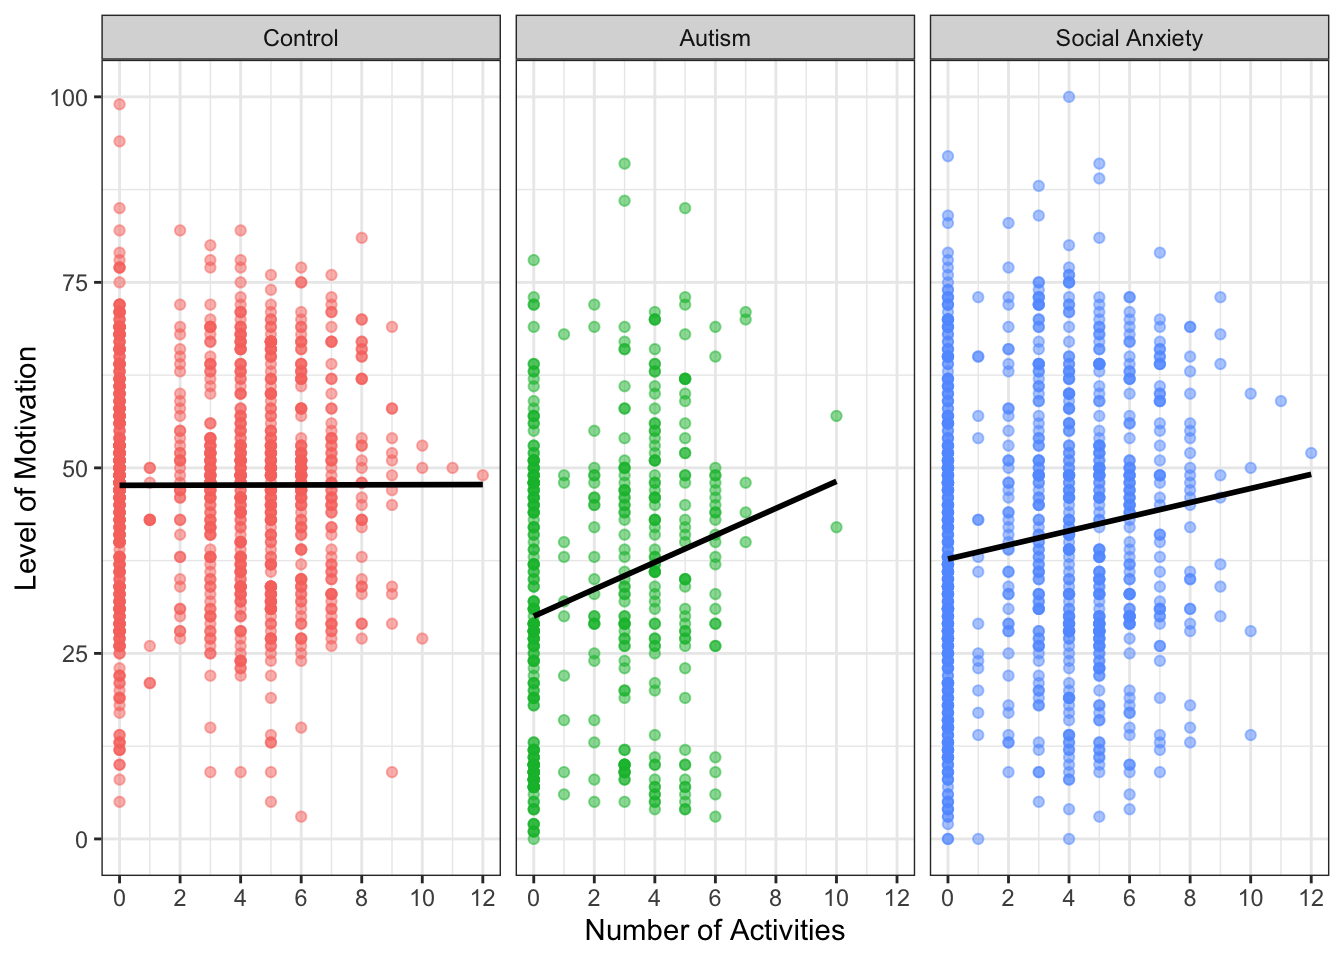
\includegraphics{04_results_files/figure-pdf/fig-Analy-1.pdf}

}

\caption{\label{fig-Analy}Motivation vs.~number of activities for all
three groups.}

\end{figure}%

This analysis demonstrated that without accounting for FE there is no
significant relationship between the number of activities and motivation
for the control group. Conversely, for the autism group, there is a
steep slope, indicating that as the number of activities increases, the
motivation of individuals also increases. Similarly, the social anxiety
group shows a positive slope, though less pronounced than the autism
group, suggesting that increased activities correlate with higher
motivation levels. These findings contradict expectations from existing
literature, which suggests that motivation levels in the autism and
social anxiety groups should not necessarily rise with an increase in
activities. This discrepancy highlights the importance of using the FE
model.

Figure~\ref{fig-FEAnaly} presents these plots, demonstrating how the
number of activities influences motivation. The pooling line, which is
dashed, shows what the intercept and slope would be if all of the data
was analyzed together instead of looking at each individual by using FE.
When using the FE models, individual lines of best fit are created for
each participant, shown with the individual solid lines. This means that
each individual has a different intercept, but they all have the same
slope.

\begin{figure}[H]

\centering{

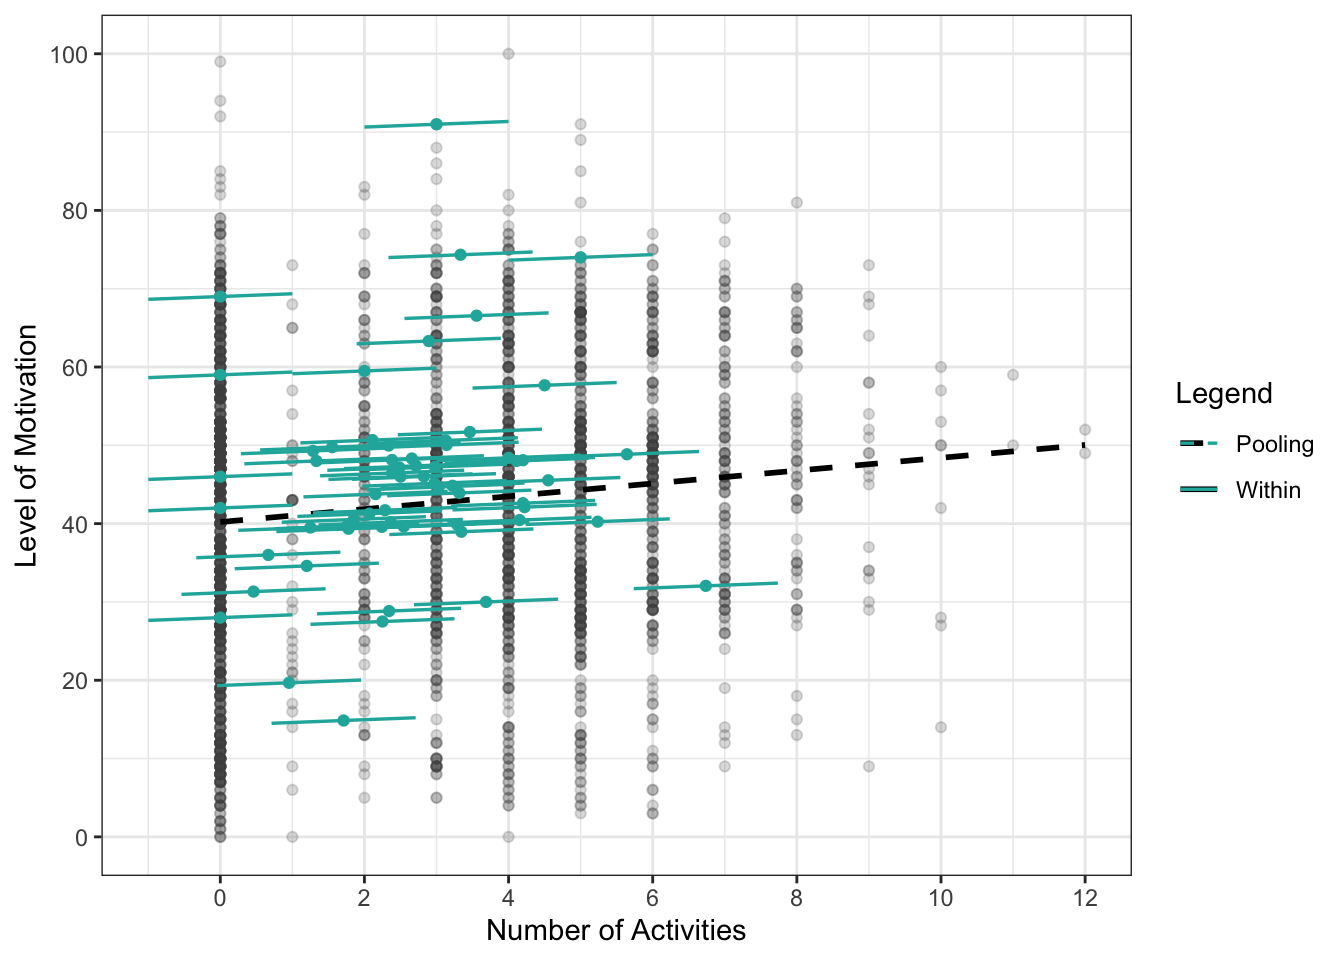
\includegraphics{04_results_files/figure-pdf/fig-FEAnaly-1.pdf}

}

\caption{\label{fig-FEAnaly}FE model for motivation vs.~number of
activities for all participants.}

\end{figure}%

While we know that it is important to model each participant
individually to account for different individual baseline levels of
motivation, we determined that applying a FE model to each
group---control, autism, and social anxiety---might be important for
understanding the true relationship between the number of activities and
motivation since each group may also have different baseline levels of
motivation.

Figure~\ref{fig-groupFE} presents the results of the FE models for all
three groups: control, autism, and social anxiety. These models predict
motivation based on the number of activities, while accounting for
individual baseline differences and well as group baseline differences.
By doing so, we can more accurately assess the impact of activities on
motivation within each distinct group. The plots highlight the unique
patterns within each group, reinforcing the importance of these tailored
analyses. The plots for both the autism group and the social anxiety
group in Figure~\ref{fig-groupFE} show steeper slopes when pooling all
of the data together, however, when the individuals are analyzed
separately, the slopes for each group are much less steep. The results
align better with our expectations based on the literature.

\begin{figure}[H]

\centering{

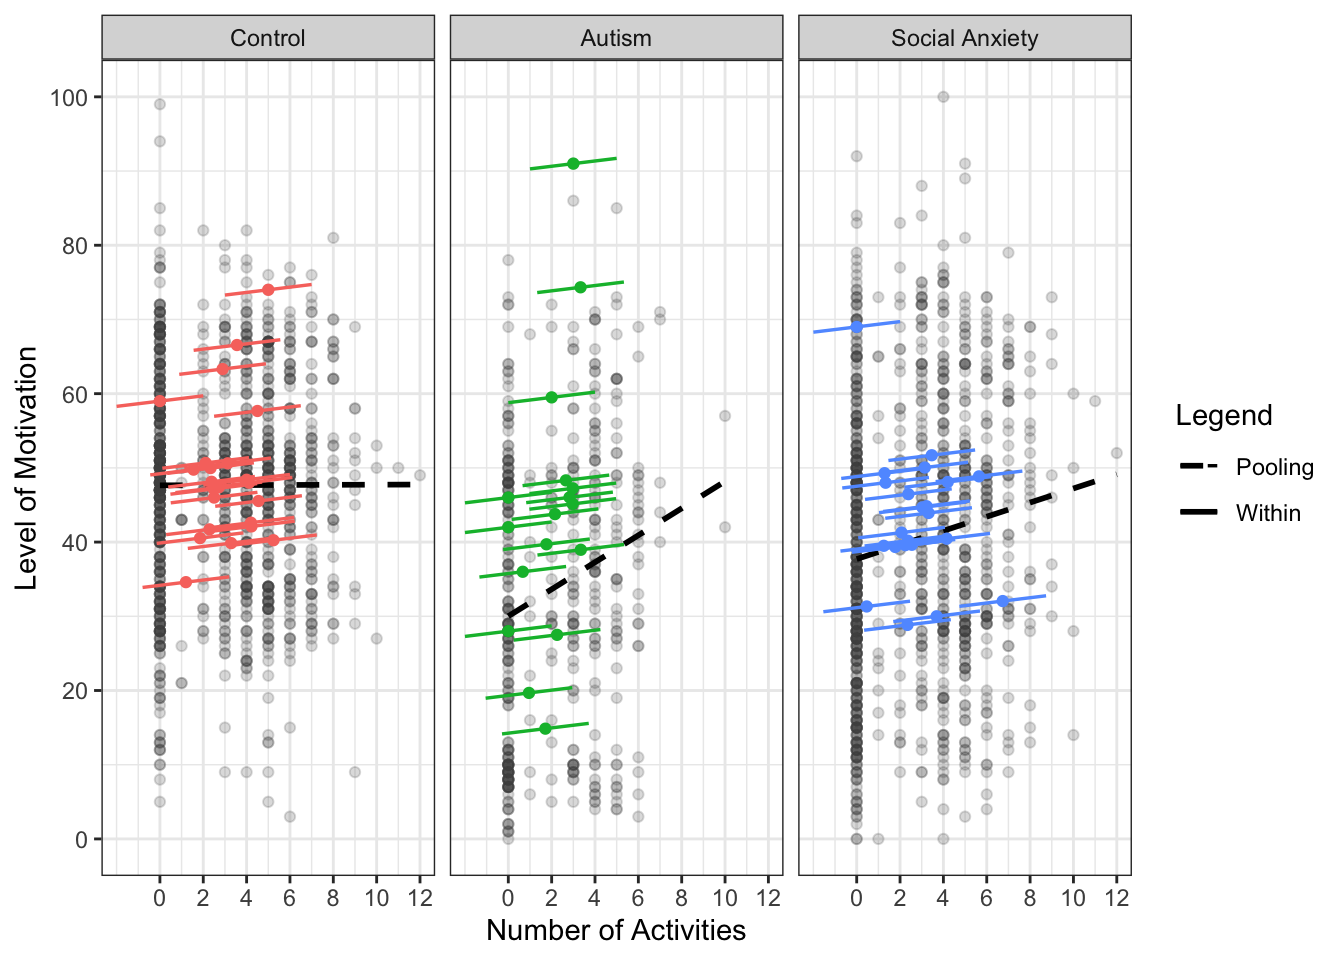
\includegraphics{04_results_files/figure-pdf/fig-groupFE-1.pdf}

}

\caption{\label{fig-groupFE}FE model for motivation vs.~number of
activities by group.}

\end{figure}%

Since these FE models rely on having both an evening survey response for
motivation and a number of activities determined by the DBSCAN-TE
algorithm, we lose some data. This loss of data reduced the number of
individuals from 31 to 23 in the control group, from 29 to 17 in the
autism group, and from 28 to 22 in the social anxiety group. The FE
models require sufficient data points for each individual to perform the
analysis effectively, which likely explains the reduction in the number
of participants for these models. After visualizing these relationships,
we proceeded to run the FE models for each group. The results from these
models are presented in Table~\ref{tbl-groupFEAnaly}.

\begin{table}

\caption{\label{tbl-groupFEAnaly}FE Models: Motivation and Number of
Activities by Group}

\centering{

\centering
\begin{tabular}[t]{lccc}
\toprule
  & Group: Control & Group: Autism & Group: Social Anxiety\\
\midrule
No. of Activities & 0.259+ & 0.361 & 0.483*\\
 & (1.716) & (1.147) & (2.149)\\
\midrule
No. of Obs. & 1,167 & 451 & 1,033\\
AIC & 9,177.454 & 3,597.049 & 8,797.231\\
R² & 0.003 & 0.003 & 0.004\\
\bottomrule
\multicolumn{4}{l}{\rule{0pt}{1em}Robust t-statistics in parentheses. + p \$<\$ 0.1, * p \$<\$ 0.05, ** p \$<\$ 0.01, *** p \$<\$ 0.001}\\
\end{tabular}

}

\end{table}%

The FE models for the control, autism, and social anxiety groups reveal
varying relationships between the number of activities and levels of
motivation. For the control group, the coefficient was 0.259, with a
marginally significant positive relationship. This suggests that, while
the number of activities may slightly increase motivation, the evidence
is not strong. In the autism group, the coefficient was 0.361 with a
positive but not statistically significant relationship between number
of activities and motivation. This indicates that an increase in
activities may correlate with higher motivation, but the evidence is not
strong enough to draw definitive conclusions. The social anxiety group
had a coefficient of 0.483 with a statistically significant positive
relationship. This suggests that an increase in the number of activities
is associated with a notable increase in motivation for individuals with
social anxiety.

Overall, these results highlight the importance of considering
individual differences in motivation across the different groups. The
significant positive relationship in the social anxiety group suggests
that interventions increasing the number of activities may be
particularly effective in boosting motivation for these individuals.
Conversely, the control and autism groups did not exhibit strong
evidence of such a relationship, indicating that other factors may play
a more crucial role in influencing motivation for these populations.

\subsubsection{Motivation and Suicidal
Ideation}\label{motivation-and-suicidal-ideation}

The prevalence of suicidal ideation across the groups underscores the
complex interplay between mental health and activity engagement. The
literature suggests that suicidal behavior is negatively associated with
overall well-being (Fonseca-Pedrero et al., 2022; Fumero et al., 2021).
Since we connected motivation to well-being, a similar association is
drawn between suicidal tendency and motivation.

Based on similar conclusions from the motivation and number of
activities analysis, we continued to perform the analysis by group.
Table~\ref{tbl-groupFESuic} shows the FE models for the impact of
suicidal intensity, which was scored from 1-100, on level of motivation,
which was also scored from 1-100, for individuals by group.

\begin{table}

\caption{\label{tbl-groupFESuic}FE Models: Motivation and Suicidal
Intensity by Group}

\centering{

\centering
\begin{talltblr}[         %% tabularray outer open
entry=none,label=none,
note{}={Robust t-statistics in parentheses. + p < 0.1, * p < 0.05, ** p < 0.01, *** p < 0.001},
]                     %% tabularray outer close
{                     %% tabularray inner open
colspec={Q[]Q[]Q[]Q[]},
column{1}={halign=l,},
column{2}={halign=c,},
column{3}={halign=c,},
column{4}={halign=c,},
hline{4}={1,2,3,4}{solid, 0.05em, black},
}                     %% tabularray inner close
\toprule
& Group: Autism & Group: Social Anxiety & Group: Control \\ \midrule %% TinyTableHeader
Suicidal Intesity & -0.095+   & -0.160*** & -0.361** \\
& (-1.927)  & (-5.518)  & (-3.293) \\
No. of Obs.       & 484       & 822       & 66       \\
AIC               & 3,942.104 & 6,934.607 & 568.685  \\
R²                & 0.012     & 0.04      & 0.113    \\
\bottomrule
\end{talltblr}

}

\end{table}%

The FE models for individuals in the autism, social anxiety, and control
groups reveal distinct relationships between suicidal intensity and
motivation levels. In the autism group, the coefficient for suicidal
intensity is -0.095, indicating a marginally significant negative
relationship. This suggests that higher levels of suicidal intensity may
slightly decrease motivation, although the evidence is not robust.
Conversely, in the social anxiety group, the coefficient is -0.160, with
a statistically significant negative relationship. This suggests that
higher levels of suicidal intensity are strongly associated with
decreased motivation among individuals with social anxiety. Similarly,
in the control group, the coefficient is -0.361, with a statistically
significant negative relationship. This suggests that higher levels of
suicidal intensity are significantly associated with reduced motivation
among individuals in the control group.

Overall, these results highlight the importance of considering the
impact of suicidal intensity on motivation levels within different
groups. While the associations are significant across all groups, the
strength and significance of the relationship varies, underscoring the
need for tailored interventions to address motivational challenges in
each population.

\subsection{Activity Types}\label{activity-types}

We investigated the impact of activity numbers at various locations on
motivation levels across each group. Analyzed locations included parks,
grocery stores, libraries, and social recreation spaces. The analysis
factored in activity counts determined by the DBSCAN-TE algorithm, along
with seven-day and 14-day moving averages. While all activity locations
and measurements were included, only a few yielded statistically
significant results. Notably, significant findings emerged for the
seven-day average park activities and daily grocery store activities.

\subsubsection{Activities at Parks}\label{activities-at-parks}

Table~\ref{tbl-groupFEParks} presents the FE models for the seven-day
rolling average number of activities at parks for the three groups.

\begin{table}

\caption{\label{tbl-groupFEParks}FE Models: Motivation and Number of
Activities at Parks by Group}

\centering{

\centering
\resizebox{\ifdim\width>\linewidth 1\linewidth\else\width\fi}{!}{
\begin{talltblr}[         %% tabularray outer open
entry=none,label=none,
note{}={Robust t-statistics in parentheses. + p < 0.1, * p < 0.05, ** p < 0.01, *** p < 0.001},
]                     %% tabularray outer close
{                     %% tabularray inner open
colspec={Q[]Q[]Q[]Q[]},
column{1}={halign=l,},
column{2}={halign=c,},
column{3}={halign=c,},
column{4}={halign=c,},
hline{4}={1,2,3,4}{solid, 0.05em, black},
}                     %% tabularray inner close
\toprule
& Group: Control & Group: Autism & Group: Social Anxiety \\ \midrule %% TinyTableHeader
Seven-Day Park & 3.017*    & 4.938     & 1.511     \\
& (2.239)   & (0.857)   & (0.207)   \\
No. of Obs.    & 1,840     & 774       & 1,597     \\
AIC            & 14,509.34 & 6,215.856 & 13,615.11 \\
R²             & 0.002     & 0.001     & 0         \\
\bottomrule
\end{talltblr}
}

}

\end{table}%

In examining park activities, statistically significant results were
observed solely for the control group. A positive correlation emerged,
indicating that each additional park activity within a seven-day period
corresponded with a 3.017-point increase in motivation score. This
suggests that frequent park visits over a week are linked to heightened
motivation levels among individuals in the control group. Conversely,
the analysis did not unveil any significant correlation between park
visits and motivation levels for the autism and social anxiety groups.
This implies that park activities within the examined time frames do not
notably affect motivation levels for these groups.

\subsubsection{Activities at Grocery
Stores}\label{activities-at-grocery-stores}

Table~\ref{tbl-groupFEGrocery} presents the FE models for the number of
activities at grocery stores for the three groups.

\begin{table}

\caption{\label{tbl-groupFEGrocery}FE Models: Motivation and Number of
Activities at Grocery Stores by Group}

\centering{

\centering
\resizebox{\ifdim\width>\linewidth 1\linewidth\else\width\fi}{!}{
\begin{talltblr}[         %% tabularray outer open
entry=none,label=none,
note{}={Robust t-statistics in parentheses. + p < 0.1, * p < 0.05, ** p < 0.01, *** p < 0.001},
]                     %% tabularray outer close
{                     %% tabularray inner open
colspec={Q[]Q[]Q[]Q[]},
column{1}={halign=l,},
column{2}={halign=c,},
column{3}={halign=c,},
column{4}={halign=c,},
hline{4}={1,2,3,4}{solid, 0.05em, black},
}                     %% tabularray inner close
\toprule
& Group: Control & Group: Autism & Group: Social Anxiety \\ \midrule %% TinyTableHeader
Grocery Store & -2.690+   & -2.725*** & 0.519     \\
& (-1.878)  & (-3.721)  & (0.614)   \\
No. of Obs.   & 1,167     & 451       & 1,033     \\
AIC           & 9,178.666 & 3,598.227 & 8,801.453 \\
R²            & 0.002     & 0.001     & 0         \\
\bottomrule
\end{talltblr}
}

}

\end{table}%

The examination of grocery store visits unveiled intriguing trends
across the different groups. Notably, a statistically significant
negative correlation was found for the autism group, indicating a
decrease in motivation by 2.725 points with each additional grocery
store activity (p \textless{} 0.001). Similarly, the control group
exhibited a slight negative correlation (p \textless{} 0.1), with each
additional daily extra grocery store visit reducing motivation by 2.690
points. Conversely, no statistical significance was observed for the
social anxiety group. These findings underscore a nuanced connection
between grocery store visits and motivation, with notable negative
impacts identified in the autism group, while no significant
associations were evident in the control and social anxiety groups.

\subsubsection{Activity Impact on
Motivation}\label{activity-impact-on-motivation}

These findings matter because they highlight the different ways in which
activities influence the mental well-being of individuals with autism,
social anxiety, and those without these conditions. The significant
correlations for the control group in seven-day average park visits
suggest that engaging in outdoor activities can be beneficial for
general well-being, while the negative correlations for grocery visits
underscore the potential stressors associated with routine tasks for
those with autism. Understanding these differences is crucial for
developing tailored interventions. For instance, enhancing access to and
encouraging regular visits to parks might improve well-being for the
general population, while reducing stressors in grocery store
environments could benefit autistic individuals. The lack of significant
findings related to specific activity locations for the social anxiety
group suggests that other factors may be more influential in their
well-being, such as engaging in more activities overall and not
necessarily activities at specific types of locations.

\bookmarksetup{startatroot}

\section{Conclusions}\label{conclusions}

This study has provided valuable insights into the complex relationship
between travel behavior and mental health among young adults with
suicidal ideation. By analyzing LBS data and conducting statistical
modeling, we uncovered significant differences in activity engagement,
motivation levels, and suicidal ideation across different neurological
or physiological groups.

\subsection{Overall Implications}\label{overall-implications}

In this study, we explored the distinct differences in activity
engagement, motivation levels, and suicidal tendencies among individuals
in autism, social anxiety, and control groups to better understand the
unique challenges these populations face.

The study revealed that autistic individuals and individuals with social
anxiety engage in fewer activities compared to the control group,
indicating unique challenges in their daily routines and social
interactions. It also showed that motivation levels are lower in both
the autism and social anxiety groups compared to the control group,
highlighting the significant impact these conditions have on personal
drive. Specifically, the control group exhibited the highest motivation
levels, followed by the autism group, with the social anxiety group
having the lowest. Additionally, a correlation was found between
increased suicidal intensity and decreased motivation across all groups,
with the social anxiety group reporting the highest frequency of
suicidal thoughts.

We also identified a minimal positive relationship between the number of
activities and motivation, suggesting that simply increasing activity
engagement is not enough to significantly enhance motivation. Moreover,
a negative relationship between travel distance and motivation was
observed, indicating that longer travel distances slightly decrease
motivation, though the effect is relatively minor. Ultimately, adjusting
either of these aspects of travel would not be a sufficient strategy for
significantly boosting motivation for individuals.

Overall, these findings highlight significant differences in activity
engagement, motivation levels, and suicidality among individuals with
autism, social anxiety, and the control group. They underscore the need
for tailored approaches to address the unique challenges faced by each
group.

\subsection{Group Specific
Implications}\label{group-specific-implications}

Different types of activities had varying effects on motivation levels
across the groups studied. For individuals with social anxiety, a
positive relationship was observed between the number of activities
engaged in and their motivation levels, indicating that increased
activity participation could enhance their well-being. Conversely, for
autistic individuals, there was a negative correlation between grocery
store visits and motivation levels, suggesting that grocery store
environments may present stressors that adversely affect their
well-being. These findings are important as they provide insight into
the distinct challenges faced by individuals with social anxiety and
autism. Additionally, the strong positive correlation between seven-day
average park visits and motivation levels in the control group
highlights the beneficial impact of outdoor green-space activities on
well-being.

In summary, each group benefits differently from various activities,
underscoring the importance of personalized approaches to improving
well-being tailored to the specific needs and preferences of individuals
in each group.

\subsection{Significance}\label{significance}

In this research, we explored the critical link between travel behavior
and mental health, focusing on young adults with suicidal ideation. By
analyzing daily activities and movement patterns, the study highlights
the importance of considering these factors in mental health
interventions. The contributions of this work bridge the gap between
travel behavior and mental health research, emphasizing the need for
personalized approaches that take into account the unique challenges
faced by individuals with autism and social anxiety.

The study reveals that individuals with autism and social anxiety engage
in fewer activities and have lower motivation levels compared to the
control group, underscoring the significant impact of these conditions
on daily life. Additionally, the correlation between suicidal ideation
and decreased motivation across all groups highlights critical areas for
intervention and prevention.

The practical implications of these findings are significant. By
understanding how travel behavior influences motivation levels and
well-being, mental health practitioners can develop targeted strategies
to support individuals struggling with mental health challenges. For
example, interventions can be tailored to address specific needs related
to travel patterns, such as mitigating stressors in grocery store
environments for autistic individuals or encouraging activity engagement
for those with social anxiety.

Overall, this research underscores the importance of considering travel
behavior as a key factor in promoting mental well-being. It offers a
roadmap for future studies to explore this intersection further,
ultimately aiming to enhance the quality of life for individuals by
informing more personalized and effective mental health strategies.

\bookmarksetup{startatroot}

\section{Limitations and Future
Recommendations}\label{limitations-and-future-recommendations}

There are some important limitations and future considerations following
the analysis of the BYU CAPS data. These limitations are due to
potential issues with data collection, lack of activities duration from
the DBSCAN-TE algorithm, and the inability to confirm activity
engagement for the participants.

\subsection{Data Collection}\label{data-collection}

The primary limitation of this study pertains to the quality of the data
of the participants. Since participants participated for varying lengths
of time and their phones were not always on to collect LBS data, the
data was sometimes sparse. Even though a substantial amount of data had
to be discarded due to poor quality, influenced by factors such as
participants turning off their phones or the app failing to record data
accurately, we did our best to accurately account for the well-being and
activity patterns of the individuals. The inconsistency in data
collection may have made it difficult for the DBSCAN-TE algorithm to
perfectly identify activities. While it performed with 91.5\% accuracy,
some of the activity days that were manually checked appeared to be
missing identified activities. Additionally, since the userID-activity
days needed corresponding mental health data and activity data, we tried
to account for the gaps by imputing the number of activities for a
seven-day rolling average number of activities and by calculating the
convex hull area and the distance traveled.

To address these limitations in future studies, improving data quality
would be paramount. Strategies could include implementing measures to
encourage consistent phone usage among participants or enhancing the
app's reliability in recording data accurately. Additionally,
incorporating redundancy measures within the data collection process,
such as cross-referencing data from multiple sources or employing
complementary data collection methods, could help mitigate the impact of
sporadic data collection. Moreover, refining the DBSCAN-TE algorithm to
improve accuracy in identifying activities, potentially through machine
learning techniques or incorporating additional contextual information,
could enhance the reliability of activity data. By prioritizing efforts
to enhance data quality and implementing more robust data collection and
processing procedures, future studies can better capture and analyze
individuals' mental health and activity patterns, thereby yielding
additional findings.

\subsection{Activity Duration}\label{activity-duration}

The study also lacks detailed information on the duration of
participants' activities. While the dataset indicates that certain
activities occurred, it does not specify how long participants spent
engaging in these activities. For example, we know whether participants
visited parks, but not the duration of their stay at the park. This
limitation means we cannot accurately assess the impact of time spent in
specific environments on mental well-being. Additionally, since the
algorithm determined activities based on relatively stationary LBS data,
we did not account for instances where participants might have merely
passed through green-spaces or parks without spending significant time
there. This omission further complicates our understanding of the
relationship between activities and mental health. These limitations
highlight the challenges in using mobile-based data collection for
mental health research.

Future studies could focus on improving the accuracy of
location-tracking algorithms, ensuring consistent data collection, and
capturing detailed activity duration to provide a more comprehensive
understanding of the interaction between travel behavior and mental
well-being.

\subsection{Activity Diaries}\label{activity-diaries}

One other potential limitation of our study is the inability to confirm
which specific activities individuals participated in throughout the
day. While we have identified activities using the DBSCAN-TE algorithm,
there is a possibility that certain activities were not accurately
identified by the algorithm, leading to their omission from our
analysis. This lack of precision could potentially result in some
activities going undetected, thereby limiting the comprehensiveness of
our activity analysis.

To address this limitation in future research, integrating activity
diaries into survey methodology could prove beneficial. By incorporating
activity diaries, participants would have the opportunity to provide
detailed accounts of their daily activities, including specific
locations where these activities took place. This additional information
could enhance the completeness and accuracy of our activity analysis, as
it would provide valuable insights into the types and locations of
activities individuals engage in throughout the day.

\subsection{Overall Recommendations}\label{overall-recommendations}

To build on the findings of this study and address its limitations,
future research should prioritize the following:

\begin{itemize}
\item
  Enhance Data Collection Methods: Consider using multiple data sources
  or complementary methods to ensure comprehensive data capture. Invest
  in refining activity identification algorithms and explore advanced
  machine learning techniques to improve accuracy and reduce gaps in
  activity data.
\item
  Capture Detailed Activity Duration: Focus on capturing both activity
  types and durations by implementing time-tracking features to better
  understand the impact of activities on mental well-being.
\item
  Implement Participant Activity Diaries: Integrate activity diaries to
  confirm activity engagement and duration. Enhance the completeness and
  accuracy of daily activity engagement.
\end{itemize}

By addressing these recommendations, future studies can improve the
quality of data, enhance the accuracy of activity analysis, and provide
a more comprehensive understanding of the interplay between activity
patterns and mental health.

\bookmarksetup{startatroot}

\section*{Acknowledgments}\label{acknowledgments}
\addcontentsline{toc}{section}{Acknowledgments}

\markboth{Acknowledgments}{Acknowledgments}

This data used in this research was collected with help from an
Interdisciplinary Research Grant at Brigham Young University, and
administered under IRB protocol F2020-242. The investigators on the
overarching grant include Terisa Gabrielsen, Jared Nielsen, and Mikle
South.

\bookmarksetup{startatroot}

\section*{References}\label{references}
\addcontentsline{toc}{section}{References}

\markboth{References}{References}

\phantomsection\label{refs}
\begin{CSLReferences}{1}{0}
\bibitem[\citeproctext]{ref-aylottExploratoryStudyGrocery1998}
Aylott, R., \& Mitchell, V.-W. (1998). An exploratory study of grocery
shopping stressors. \emph{International Journal of Retail \&
Distribution Management}, \emph{26}(9), 362--373.
\url{https://doi.org/10.1108/09590559810237908}

\bibitem[\citeproctext]{ref-baileyRelationshipSocialExperience2020}
Bailey, K. M., Frost, K. M., Casagrande, K., \& Ingersoll, B. (2020).
The relationship between social experience and subjective well-being in
autistic college students: {A} mixed methods study. \emph{Autism},
\emph{24}(5), 1081--1092. \url{https://doi.org/10.1177/1362361319892457}

\bibitem[\citeproctext]{ref-barryAddressingDeterminantsPositive2009}
Barry, M. M. (2009). Addressing the determinants of positive mental
health: {Concepts}, evidence and practice. \emph{International Journal
of Mental Health Promotion}, \emph{11}(3), 4--17.
\url{https://doi.org/10.1080/14623730.2009.9721788}

\bibitem[\citeproctext]{ref-bowlerSystematicReviewEvidence2010}
Bowler, D. E., Buyung-Ali, L. M., Knight, T. M., \& Pullin, A. S.
(2010). A systematic review of evidence for the added benefits to health
of exposure to natural environments. \emph{BMC Public Health},
\emph{10}(1), 456. \url{https://doi.org/10.1186/1471-2458-10-456}

\bibitem[\citeproctext]{ref-bratmanNatureExperienceReduces2015}
Bratman, G. N., Hamilton, J. P., Hahn, K. S., Daily, G. C., \& Gross, J.
J. (2015). Nature experience reduces rumination and subgenual prefrontal
cortex activation. \emph{Proceedings of the National Academy of
Sciences}, \emph{112}(28), 8567--8572.
\url{https://doi.org/10.1073/pnas.1510459112}

\bibitem[\citeproctext]{ref-brewsterPublicLibraryTherapeutic2014}
Brewster, L. (2014). The public library as therapeutic landscape: {A}
qualitative case study. \emph{Health \& Place}, \emph{26}, 94--99.
\url{https://doi.org/10.1016/j.healthplace.2013.12.015}

\bibitem[\citeproctext]{ref-dekaTravelPatternsNeeds2016}
Deka, D., Feeley, C., \& Lubin, A. (2016). Travel patterns, needs, and
barriers of adults with autism spectrum disorder: {Report} from a
survey. \emph{Transportation Research Record}, \emph{2542}(1), 9--16.
\url{https://doi.org/10.3141/2542-02}

\bibitem[\citeproctext]{ref-delboscExploringRelativeInfluences2011}
Delbosc, A., \& Currie, G. (2011). Exploring the relative influences of
transport disadvantage and social exclusion on well-being.
\emph{Transport Policy}, \emph{18}(4), 555--562.
\url{https://doi.org/10.1016/j.tranpol.2011.01.011}

\bibitem[\citeproctext]{ref-eliaPublicLibrariesSupporting2019}
Elia, H. (2019). Public libraries supporting health and wellness: {A}
literature review. \emph{School of Information Student Research
Journal}, \emph{9}(2). \url{https://doi.org/10.31979/2575-2499.090207}

\bibitem[\citeproctext]{ref-fonseca-pedreroRiskProtectiveFactors2022}
Fonseca-Pedrero, E., Al-Halabí, S., Pérez-Albéniz, A., \& Debbané, M.
(2022). Risk and protective factors in adolescent suicidal behaviour:
{A} network analysis. \emph{International Journal of Environmental
Research and Public Health}, \emph{19}(3), 1784.
\url{https://doi.org/10.3390/ijerph19031784}

\bibitem[\citeproctext]{ref-frimanHowDoesTravel2017}
Friman, M., Gärling, T., Ettema, D., \& Olsson, L. E. (2017). How does
travel affect emotional well-being and life satisfaction?
\emph{Transportation Research Part A: Policy and Practice}, \emph{106},
170--180. \url{https://doi.org/10.1016/j.tra.2017.09.024}

\bibitem[\citeproctext]{ref-fumeroAdolescentsBipolarExperiences2021}
Fumero, A., Marrero, R. J., Pérez-Albéniz, A., \& Fonseca-Pedrero, E.
(2021). Adolescents' bipolar experiences and suicide risk: {Well-being}
and mental health difficulties as mediators. \emph{International Journal
of Environmental Research and Public Health}, \emph{18}(6), 3024.
\url{https://doi.org/10.3390/ijerph18063024}

\bibitem[\citeproctext]{ref-gasconLongtermExposureResidential2018}
Gascon, M., Sánchez-Benavides, G., Dadvand, P., Martínez, D., Gramunt,
N., Gotsens, X., Cirach, M., Vert, C., Molinuevo, J. L., Crous-Bou, M.,
\& Nieuwenhuijsen, M. (2018). Long-term exposure to residential green
and blue spaces and anxiety and depression in adults: {A}
cross-sectional study. \emph{Environmental Research}, \emph{162},
231--239. \url{https://doi.org/10.1016/j.envres.2018.01.012}

\bibitem[\citeproctext]{ref-kennyWhichTermsShould2016}
Kenny, L., Hattersley, C., Molins, B., Buckley, C., Povey, C., \&
Pellicano, E. (2016). Which terms should be used to describe autism?
{Perspectives} from the {UK} autism community. \emph{Autism},
\emph{20}(4), 442--462. \url{https://doi.org/10.1177/1362361315588200}

\bibitem[\citeproctext]{ref-kuykendallLeisureEngagementSubjective2015}
Kuykendall, L., Tay, L., \& Ng, V. (2015). Leisure engagement and
subjective well-being: {A} meta-analysis. \emph{Psychological Bulletin},
\emph{141}(2), 364--403. \url{https://doi.org/10.1037/a0038508}

\bibitem[\citeproctext]{ref-lanDailySpacetimeActivities2022}
Lan, Y., Roberts, H., Kwan, M.-P., \& Helbich, M. (2022). Daily
space-time activities, multiple environmental exposures, and anxiety
symptoms: {A} cross-sectional mobile phone-based sensing study.
\emph{Science of The Total Environment}, \emph{834}, 155276.
\url{https://doi.org/10.1016/j.scitotenv.2022.155276}

\bibitem[\citeproctext]{ref-leichsenringSocialAnxietyDisorder2017}
Leichsenring, F., \& Leweke, F. (2017). Social anxiety disorder.
\emph{New England Journal of Medicine}, \emph{376}(23), 2255--2264.
\url{https://doi.org/10.1056/NEJMcp1614701}

\bibitem[\citeproctext]{ref-loadesRapidSystematicReview2020}
Loades, M. E., Chatburn, E., Higson-Sweeney, N., Reynolds, S., Shafran,
R., Brigden, A., Linney, C., McManus, M. N., Borwick, C., \& Crawley, E.
(2020). Rapid systematic review: {The} impact of social isolation and
loneliness on the mental health of children and adolescents in the
context of {COVID-19}. \emph{Journal of the American Academy of Child \&
Adolescent Psychiatry}, \emph{59}(11), 1218--1239.e3.
\url{https://doi.org/10.1016/j.jaac.2020.05.009}

\bibitem[\citeproctext]{ref-lubinTransportationIssuesAdults2016}
Lubin, A., \& Feeley, C. (2016). Transportation issues of adults on the
autism spectrum: {Findings} from focus group discussions.
\emph{Transportation Research Record}, \emph{2542}(1), 1--8.
\url{https://doi.org/10.3141/2542-01}

\bibitem[\citeproctext]{ref-macfarlaneClassifyingLocationPoints2024}
Macfarlane, G. S., Riches, G., Youngs, E. K., \& Nielsen, J. A. (2024).
Classifying location points as daily activities using simultaneously
optimized {DBSCAN-TE} parameters. \emph{Findings}.
\url{https://doi.org/10.32866/001c.116197}

\bibitem[\citeproctext]{ref-mackettMentalHealthTravel2021}
Mackett, R. L. (2021). Mental health and travel behaviour. \emph{Journal
of Transport \& Health}, \emph{22}, 101143.
\url{https://doi.org/10.1016/j.jth.2021.101143}

\bibitem[\citeproctext]{ref-MentalHealthNumbers2023}
Mental {Health By} the {Numbers}. (2023). In \emph{NAMI}.

\bibitem[\citeproctext]{ref-nilssonEffectsTimePressure2017}
Nilsson, E., Gärling, T., \& Marell, A. (2017). Effects of time
pressure, type of shopping, and store attributes on consumers'
satisfaction with grocery shopping. \emph{The International Review of
Retail, Distribution and Consumer Research}, \emph{27}(4), 334--351.
\url{https://doi.org/10.1080/09593969.2017.1309674}

\bibitem[\citeproctext]{ref-orbenEffectsSocialDeprivation2020}
Orben, A., Tomova, L., \& Blakemore, S.-J. (2020). The effects of social
deprivation on adolescent development and mental health. \emph{The
Lancet Child \& Adolescent Health}, \emph{4}(8), 634--640.
\url{https://doi.org/10.1016/S2352-4642(20)30186-3}

\bibitem[\citeproctext]{ref-ozturkRelationshipAttachmentStyle2010}
Öztürk, A., \& Mutlu, T. (2010). The relationship between attachment
style, subjective well-being, happiness and social anxiety among
university students'. \emph{Procedia - Social and Behavioral Sciences},
\emph{9}, 1772--1776. \url{https://doi.org/10.1016/j.sbspro.2010.12.398}

\bibitem[\citeproctext]{ref-pelgrimsAssociationUrbanEnvironment2021}
Pelgrims, I., Devleesschauwer, B., Guyot, M., Keune, H., Nawrot, T. S.,
Remmen, R., Saenen, N. D., Trabelsi, S., Thomas, I., Aerts, R., \& De
Clercq, E. M. (2021). Association between urban environment and mental
health in {Brussels}, {Belgium}. \emph{BMC Public Health}, \emph{21}(1),
635. \url{https://doi.org/10.1186/s12889-021-10557-7}

\bibitem[\citeproctext]{ref-pousoContactBluegreenSpaces2021}
Pouso, S., Borja, Á., Fleming, L. E., Gómez-Baggethun, E., White, M. P.,
\& Uyarra, M. C. (2021). Contact with blue-green spaces during the
{COVID-19} pandemic lockdown beneficial for mental health. \emph{Science
of The Total Environment}, \emph{756}, 143984.
\url{https://doi.org/10.1016/j.scitotenv.2020.143984}

\bibitem[\citeproctext]{ref-rateringMovingAnxietyDisorder2024}
Ratering, C., van der Heijden, R., \& Martens, K. (2024). Moving around
with an anxiety disorder. \emph{Transportation Research Part F: Traffic
Psychology and Behaviour}, \emph{100}, 493--506.
\url{https://doi.org/10.1016/j.trf.2023.12.005}

\bibitem[\citeproctext]{ref-rautioLivingEnvironmentIts2018}
Rautio, N., Filatova, S., Lehtiniemi, H., \& Miettunen, J. (2018).
Living environment and its relationship to depressive mood: {A}
systematic review. \emph{International Journal of Social Psychiatry},
\emph{64}(1), 92--103. \url{https://doi.org/10.1177/0020764017744582}

\bibitem[\citeproctext]{ref-richesTransformingGPSPoints2022}
Riches, G. (2022). \emph{Transforming {GPS} points to daily activities
using simultaneously optimized {DBSCAN-TE} parameters}. MS Thesis,
Brigham Young University.

\bibitem[\citeproctext]{ref-ridgwaySubjectiveWellbeingAutistic}
Ridgway, K., Macmillan, C., Demmer, D. H., Hooley, M., Hedley, D.,
Westrupp, E., \& Stokes, M. A. (2024). Subjective wellbeing of autistic
adolescents and young adults: {A} cross sectional study. \emph{Autism
Research}, \emph{n/a}(n/a). \url{https://doi.org/10.1002/aur.3139}

\bibitem[\citeproctext]{ref-roeGreenSpaceStress2013}
Roe, J. J., Thompson, C. W., Aspinall, P. A., Brewer, M. J., Duff, E.
I., Miller, D., Mitchell, R., \& Clow, A. (2013). Green space and
stress: {Evidence} from cortisol measures in deprived urban communities.
\emph{International Journal of Environmental Research and Public
Health}, \emph{10}(9), 4086--4103.
\url{https://doi.org/10.3390/ijerph10094086}

\bibitem[\citeproctext]{ref-stanleyMobilitySocialExclusion2011}
Stanley, J. K., Hensher, D. A., Stanley, J. R., \& Vella-Brodrick, D.
(2011). Mobility, social exclusion and well-being: {Exploring} the
links. \emph{Transportation Research Part A: Policy and Practice},
\emph{45}(8), 789--801. \url{https://doi.org/10.1016/j.tra.2011.06.007}

\bibitem[\citeproctext]{ref-sugiyamaAssociationsNeighbourhoodGreenness2008}
Sugiyama, T., Leslie, E., Giles-Corti, B., \& Owen, N. (2008).
Associations of neighbourhood greenness with physical and mental health:
{Do} walking, social coherence and local social interaction explain the
relationships? \emph{Journal of Epidemiology and Community Health},
\emph{62}, e9. \url{https://doi.org/10.1136/jech.2007.064287}

\bibitem[\citeproctext]{ref-syahputriEffectTravelSatisfaction2022}
Syahputri, J., Dharmowijoyo, D. B. E., Basuki Joewono, T., \& Rizki, M.
(2022). Effect of travel satisfaction and heterogeneity of
activity-travel patterns of other persons in the household on social and
mental health: {The} case of {Bandung Metropolitan} area. \emph{Case
Studies on Transport Policy}, \emph{10}(4), 2111--2124.
\url{https://doi.org/10.1016/j.cstp.2022.09.005}

\bibitem[\citeproctext]{ref-takiguchiRelationshipLeisureActivities2022}
Takiguchi, Y., Matsui, M., Kikutani, M., \& Ebina, K. (2022). The
relationship between leisure activities and mental health: {The} impact
of resilience and {COVID}-19. \emph{Applied Psychology. Health and
Well-Being}, 10.1111/aphw.12394.
\url{https://doi.org/10.1111/aphw.12394}

\bibitem[\citeproctext]{ref-timmermansSpatialContextComplexity2003}
Timmermans, H., van der Waerden, P., Alves, M., Polak, J., Ellis, S.,
Harvey, A. S., Kurose, S., \& Zandee, R. (2003). Spatial context and the
complexity of daily travel patterns: An international comparison.
\emph{Journal of Transport Geography}, \emph{11}(1), 37--46.
\url{https://doi.org/10.1016/S0966-6923(02)00050-9}

\bibitem[\citeproctext]{ref-whiteAssociationsGreenBlue2021}
White, M. P., Elliott, L. R., Grellier, J., Economou, T., Bell, S.,
Bratman, G. N., Cirach, M., Gascon, M., Lima, M. L., Lõhmus, M.,
Nieuwenhuijsen, M., Ojala, A., Roiko, A., Schultz, P. W., van den Bosch,
M., \& Fleming, L. E. (2021). Associations between green/blue spaces and
mental health across 18 countries. \emph{Scientific Reports},
\emph{11}(1), 8903. \url{https://doi.org/10.1038/s41598-021-87675-0}

\bibitem[\citeproctext]{ref-wooldridgeIntroductoryEconometricsModern2009}
Wooldridge, J. (2009). \emph{Introductory {Econometrics}: {A Modern
Appraoch}} (4th ed.). South-Western Cengage Learning. Mason, Ohio.

\bibitem[\citeproctext]{ref-yanosNegativeSupportiveSocial2001}
Yanos, P. T., Rosenfield, S., \& Horwitz, A. V. (2001). Negative and
supportive social interactions and quality of life among persons
diagnosed with severe mental illness. \emph{Community Mental Health
Journal}, \emph{37}(5), 405--419.
\url{https://doi.org/10.1023/A:1017528029127}

\bibitem[\citeproctext]{ref-yeSocialAnxietySubjective2021}
Ye, B., Li, L., Wang, P., Wang, R., Liu, M., Wang, X., \& Yang, Q.
(2021). Social anxiety and subjective well-being among {Chinese} college
students: {A} moderated mediation model. \emph{Personality and
Individual Differences}, \emph{175}, 110680.
\url{https://doi.org/10.1016/j.paid.2021.110680}

\bibitem[\citeproctext]{ref-zanalabidinSystematicLiteratureReview2023}
Zanal Abidin, N. S., Shaifuddin, N., \& Wan Mohd Saman, W. S. (2023).
Systematic literature review of the bibliotherapy practices in public
libraries in supporting communities' mental health and wellbeing.
\emph{Public Library Quarterly}, \emph{42}(2), 124--140.
\url{https://doi.org/10.1080/01616846.2021.2009291}

\end{CSLReferences}




\end{document}
